\documentclass[11pt]{ctexart}
% Shared preamble of the v4 papers (Chinese; xelatex with ctex).
\usepackage[margin=1in]{geometry}
\usepackage{amsmath,amssymb}
\usepackage{booktabs,multirow,array}
\usepackage{graphicx}
\usepackage[font=small,labelfont=bf]{caption}
\usepackage{subcaption}
\usepackage{xcolor}
\usepackage{enumitem}
\usepackage[numbers,sort&compress]{natbib}
\usepackage[hidelinks]{hyperref}
\usepackage{url}
\setlist{nosep,leftmargin=*}
\newcommand{\kev}{Kev-4B}
\newcommand{\pc}{P_{\mathrm{c}}}
\newcommand{\pg}{P_{\mathrm{g}}}
\newcommand{\ci}[2]{[#1,\,#2]}
\newenvironment{correction}{\begin{center}\begin{minipage}{0.95\linewidth}\small\setlength{\parskip}{3pt}\noindent\textbf{更正声明。}}{\end{minipage}\end{center}}

% \NUM{key}: a number computed by dcjev/analysis/paper_numbers.py and written to the paper's numbers.tex.
% A key that numbers.tex does not define prints as ??key?? and logs a warning, so a missing number cannot vanish.
\makeatletter
\newcommand{\NUM}[1]{\ifcsname num@#1\endcsname\csname num@#1\endcsname\else\textbf{??\detokenize{#1}??}\PackageWarning{numbers}{Undefined number #1}\fi}
\newcommand{\defnum}[2]{\expandafter\def\csname num@#1\endcsname{#2}}
\makeatother

% Generated by dcjev/analysis/paper_numbers.py -- do not edit.
\defnum{beh_maxdiff}{0}
\defnum{beh_runs}{165}
\defnum{dist_reacher_ar_gated}{0.253}
\defnum{dist_reacher_ar_sampled}{0.252}
\defnum{dist_reacher_env}{0.101}
\defnum{dist_reacher_env_window}{0.180}
\defnum{dist_reacher_kev_distill}{0.250}
\defnum{dist_reacher_kev_gated}{0.263}
\defnum{dist_reacher_kev_score}{0.256}
\defnum{dist_reacher_random}{0.180}
\defnum{effort_cheetah_ar_gated}{0.77}
\defnum{effort_cheetah_ar_sampled}{0.68}
\defnum{effort_cheetah_env}{0.67}
\defnum{effort_cheetah_env_window}{0.63}
\defnum{effort_cheetah_kev_distill}{0.80}
\defnum{effort_cheetah_kev_gated}{0.73}
\defnum{effort_cheetah_kev_score}{0.80}
\defnum{effort_cheetah_random}{0.33}
\defnum{effort_hopper_ar_gated}{0.89}
\defnum{effort_hopper_ar_sampled}{0.77}
\defnum{effort_hopper_env}{0.45}
\defnum{effort_hopper_env_window}{0.51}
\defnum{effort_hopper_kev_distill}{0.58}
\defnum{effort_hopper_kev_gated}{0.53}
\defnum{effort_hopper_kev_score}{0.52}
\defnum{effort_hopper_random}{0.33}
\defnum{effort_reacher_ar_gated}{0.63}
\defnum{effort_reacher_ar_sampled}{0.56}
\defnum{effort_reacher_env}{0.01}
\defnum{effort_reacher_env_window}{0.19}
\defnum{effort_reacher_kev_distill}{0.76}
\defnum{effort_reacher_kev_gated}{0.63}
\defnum{effort_reacher_kev_score}{0.36}
\defnum{effort_reacher_random}{0.33}
\defnum{effort_swimmer_ar_gated}{0.90}
\defnum{effort_swimmer_ar_sampled}{0.81}
\defnum{effort_swimmer_env}{0.61}
\defnum{effort_swimmer_env_window}{0.82}
\defnum{effort_swimmer_kev_distill}{0.87}
\defnum{effort_swimmer_kev_gated}{0.81}
\defnum{effort_swimmer_kev_score}{0.83}
\defnum{effort_swimmer_random}{0.33}
\defnum{effort_walker_ar_gated}{0.52}
\defnum{effort_walker_ar_sampled}{0.66}
\defnum{effort_walker_env}{0.59}
\defnum{effort_walker_env_window}{0.56}
\defnum{effort_walker_kev_distill}{0.56}
\defnum{effort_walker_kev_gated}{0.59}
\defnum{effort_walker_kev_score}{0.56}
\defnum{effort_walker_random}{0.33}
\defnum{fallrate_hopper}{0.08}
\defnum{fallrate_walker}{0.09}
\defnum{flip_cheetah_ar_gated}{0\%}
\defnum{flip_cheetah_ar_sampled}{0\%}
\defnum{flip_cheetah_env}{23\%}
\defnum{flip_cheetah_env_window}{59\%}
\defnum{flip_cheetah_kev_distill}{0\%}
\defnum{flip_cheetah_kev_gated}{0\%}
\defnum{flip_cheetah_kev_score}{0\%}
\defnum{flip_cheetah_random}{9\%}
\defnum{flip_maxret}{1599}
\defnum{flipruns_cheetah_ar_gated}{0}
\defnum{flipruns_cheetah_ar_sampled}{0}
\defnum{flipruns_cheetah_env}{1}
\defnum{flipruns_cheetah_env_window}{3}
\defnum{flipruns_cheetah_kev_distill}{0}
\defnum{flipruns_cheetah_kev_gated}{0}
\defnum{flipruns_cheetah_kev_score}{0}
\defnum{healthyauc_hopper_ar}{1.00}
\defnum{healthyauc_hopper_kev}{1.00}
\defnum{healthyauc_walker_ar}{1.00}
\defnum{healthyauc_walker_kev}{0.99}
\defnum{iqm_ar_gated}{0.35}
\defnum{iqm_ar_sampled}{0.31}
\defnum{iqm_env}{1.05}
\defnum{iqm_env_window}{1.10}
\defnum{iqm_kev_distill}{0.98}
\defnum{iqm_kev_gated}{1.00}
\defnum{iqm_kev_score}{0.78}
\defnum{iqmhi_ar_gated}{0.46}
\defnum{iqmhi_ar_sampled}{0.45}
\defnum{iqmhi_env}{1.16}
\defnum{iqmhi_env_window}{1.26}
\defnum{iqmhi_kev_distill}{1.10}
\defnum{iqmhi_kev_gated}{1.09}
\defnum{iqmhi_kev_score}{0.91}
\defnum{iqmlo_ar_gated}{0.28}
\defnum{iqmlo_ar_sampled}{0.19}
\defnum{iqmlo_env}{0.91}
\defnum{iqmlo_env_window}{0.89}
\defnum{iqmlo_kev_distill}{0.82}
\defnum{iqmlo_kev_gated}{0.81}
\defnum{iqmlo_kev_score}{0.60}
\defnum{judge_flipped_cheetah}{0}
\defnum{judge_runs_cheetah}{23}
\defnum{judgewin_ar_gated}{33.9k}
\defnum{judgewin_ar_sampled}{33.9k}
\defnum{judgewin_env}{0}
\defnum{judgewin_env_window}{0}
\defnum{judgewin_kev_distill}{3.5k}
\defnum{judgewin_kev_gated}{33.9k}
\defnum{judgewin_kev_score}{33.9k}
\defnum{mean_ar_gated}{0.40}
\defnum{mean_ar_sampled}{0.37}
\defnum{mean_env}{1.00}
\defnum{mean_env_window}{1.41}
\defnum{mean_kev_distill}{0.59}
\defnum{mean_kev_gated}{0.79}
\defnum{mean_kev_score}{0.76}
\defnum{median_ar_gated}{0.36}
\defnum{median_ar_sampled}{0.36}
\defnum{median_env}{1.03}
\defnum{median_env_window}{1.21}
\defnum{median_kev_distill}{1.02}
\defnum{median_kev_gated}{1.05}
\defnum{median_kev_score}{0.82}
\defnum{parity_bf16_argmax}{99.7\%}
\defnum{parity_bf16_max}{0.040}
\defnum{parity_fp32_max}{0.0009}
\defnum{parity_questions}{300}
\defnum{pimp_all_argated_arsampled}{0.49}
\defnum{pimp_all_envwindow_env}{0.54}
\defnum{pimp_all_kevdistill_env}{0.44}
\defnum{pimp_all_kevdistill_kevgated}{0.45}
\defnum{pimp_all_kevgated_argated}{0.78}
\defnum{pimp_all_kevgated_env}{0.44}
\defnum{pimp_all_kevgated_envwindow}{0.31}
\defnum{pimp_all_kevgated_kevscore}{0.55}
\defnum{pimp_all_kevscore_argated}{0.82}
\defnum{pimp_all_kevscore_env}{0.28}
\defnum{pimp_cheetah_argated_arsampled}{0.47}
\defnum{pimp_cheetah_envwindow_env}{0.20}
\defnum{pimp_cheetah_kevdistill_env}{0.72}
\defnum{pimp_cheetah_kevdistill_kevgated}{0.40}
\defnum{pimp_cheetah_kevgated_argated}{1.00}
\defnum{pimp_cheetah_kevgated_env}{0.72}
\defnum{pimp_cheetah_kevgated_envwindow}{0.92}
\defnum{pimp_cheetah_kevgated_kevscore}{1.00}
\defnum{pimp_cheetah_kevscore_argated}{0.88}
\defnum{pimp_cheetah_kevscore_env}{0.28}
\defnum{pimp_hopper_argated_arsampled}{0.53}
\defnum{pimp_hopper_envwindow_env}{0.80}
\defnum{pimp_hopper_kevdistill_env}{0.48}
\defnum{pimp_hopper_kevdistill_kevgated}{0.52}
\defnum{pimp_hopper_kevgated_argated}{1.00}
\defnum{pimp_hopper_kevgated_env}{0.44}
\defnum{pimp_hopper_kevgated_envwindow}{0.24}
\defnum{pimp_hopper_kevgated_kevscore}{0.52}
\defnum{pimp_hopper_kevscore_argated}{1.00}
\defnum{pimp_hopper_kevscore_env}{0.40}
\defnum{pimp_reacher_argated_arsampled}{0.40}
\defnum{pimp_reacher_envwindow_env}{0.00}
\defnum{pimp_reacher_kevdistill_env}{0.00}
\defnum{pimp_reacher_kevdistill_kevgated}{0.28}
\defnum{pimp_reacher_kevgated_argated}{0.48}
\defnum{pimp_reacher_kevgated_env}{0.00}
\defnum{pimp_reacher_kevgated_envwindow}{0.00}
\defnum{pimp_reacher_kevgated_kevscore}{0.12}
\defnum{pimp_reacher_kevscore_argated}{0.84}
\defnum{pimp_reacher_kevscore_env}{0.00}
\defnum{pimp_swimmer_argated_arsampled}{0.67}
\defnum{pimp_swimmer_envwindow_env}{0.92}
\defnum{pimp_swimmer_kevdistill_env}{0.64}
\defnum{pimp_swimmer_kevdistill_kevgated}{0.36}
\defnum{pimp_swimmer_kevgated_argated}{0.52}
\defnum{pimp_swimmer_kevgated_env}{0.72}
\defnum{pimp_swimmer_kevgated_envwindow}{0.20}
\defnum{pimp_swimmer_kevgated_kevscore}{0.64}
\defnum{pimp_swimmer_kevscore_argated}{0.36}
\defnum{pimp_swimmer_kevscore_env}{0.40}
\defnum{pimp_walker_argated_arsampled}{0.40}
\defnum{pimp_walker_envwindow_env}{0.80}
\defnum{pimp_walker_kevdistill_env}{0.36}
\defnum{pimp_walker_kevdistill_kevgated}{0.68}
\defnum{pimp_walker_kevgated_argated}{0.88}
\defnum{pimp_walker_kevgated_env}{0.32}
\defnum{pimp_walker_kevgated_envwindow}{0.20}
\defnum{pimp_walker_kevgated_kevscore}{0.48}
\defnum{pimp_walker_kevscore_argated}{1.00}
\defnum{pimp_walker_kevscore_env}{0.32}
\defnum{pimpenv_ar_gated}{0.18}
\defnum{pimpenv_ar_sampled}{0.12}
\defnum{pimpenv_env}{0.50}
\defnum{pimpenv_env_window}{0.54}
\defnum{pimpenv_kev_distill}{0.44}
\defnum{pimpenv_kev_gated}{0.44}
\defnum{pimpenv_kev_score}{0.28}
\defnum{pimpwin_ar_gated}{0.10}
\defnum{pimpwin_ar_sampled}{0.11}
\defnum{pimpwin_env}{0.46}
\defnum{pimpwin_env_window}{0.50}
\defnum{pimpwin_kev_distill}{0.27}
\defnum{pimpwin_kev_gated}{0.31}
\defnum{pimpwin_kev_score}{0.27}
\defnum{progress_instruction}{How well is the robot accomplishing its task in this segment?}
\defnum{rand_cheetah}{$-$280}
\defnum{rand_hopper}{13}
\defnum{rand_reacher}{$-$42}
\defnum{rand_swimmer}{$-$0.13}
\defnum{rand_walker}{$-$0.40}
\defnum{ref_hopper}{2820}
\defnum{resumed_conds}{\texttt{kev\_score}, \texttt{kev\_gated}, \texttt{kev\_distill}, \texttt{ar\_gated}}
\defnum{resumed_dropped_max}{703}
\defnum{resumed_runs}{24}
\defnum{resumed_steps}{301{,}056}
\defnum{ret_cheetah_ar_gated}{1069}
\defnum{ret_cheetah_ar_sampled}{1050}
\defnum{ret_cheetah_env}{3441}
\defnum{ret_cheetah_env_window}{2376}
\defnum{ret_cheetah_kev_distill}{4117}
\defnum{ret_cheetah_kev_gated}{4241}
\defnum{ret_cheetah_kev_score}{2845}
\defnum{ret_hopper_ar_gated}{1165}
\defnum{ret_hopper_ar_sampled}{1127}
\defnum{ret_hopper_env}{2820}
\defnum{ret_hopper_env_window}{3419}
\defnum{ret_hopper_kev_distill}{2833}
\defnum{ret_hopper_kev_gated}{3169}
\defnum{ret_hopper_kev_score}{3061}
\defnum{ret_reacher_ar_gated}{$-$75.2}
\defnum{ret_reacher_ar_sampled}{$-$68.8}
\defnum{ret_reacher_env}{$-$6.4}
\defnum{ret_reacher_env_window}{$-$28.0}
\defnum{ret_reacher_kev_distill}{$-$88.4}
\defnum{ret_reacher_kev_gated}{$-$75.8}
\defnum{ret_reacher_kev_score}{$-$48.9}
\defnum{ret_swimmer_ar_gated}{141}
\defnum{ret_swimmer_ar_sampled}{118}
\defnum{ret_swimmer_env}{81}
\defnum{ret_swimmer_env_window}{278}
\defnum{ret_swimmer_kev_distill}{91}
\defnum{ret_swimmer_kev_gated}{141}
\defnum{ret_swimmer_kev_score}{99}
\defnum{ret_walker_ar_gated}{1321}
\defnum{ret_walker_ar_sampled}{1330}
\defnum{ret_walker_env}{3150}
\defnum{ret_walker_env_window}{4068}
\defnum{ret_walker_kev_distill}{2943}
\defnum{ret_walker_kev_gated}{2536}
\defnum{ret_walker_kev_score}{2593}
\defnum{rho_cheetah_ar_gated}{0.79}
\defnum{rho_cheetah_ar_healthy}{0.76}
\defnum{rho_cheetah_ar_progress}{0.64}
\defnum{rho_cheetah_ar_progress_sampled}{0.02}
\defnum{rho_cheetah_kev_gated}{0.88}
\defnum{rho_cheetah_kev_healthy}{0.85}
\defnum{rho_cheetah_kev_progress}{0.93}
\defnum{rho_hopper_ar_gated}{0.65}
\defnum{rho_hopper_ar_healthy}{0.50}
\defnum{rho_hopper_ar_progress}{0.66}
\defnum{rho_hopper_ar_progress_sampled}{0.22}
\defnum{rho_hopper_kev_gated}{0.70}
\defnum{rho_hopper_kev_healthy}{0.56}
\defnum{rho_hopper_kev_progress}{0.73}
\defnum{rho_mean_ar_gated}{0.58}
\defnum{rho_mean_ar_healthy}{0.51}
\defnum{rho_mean_ar_progress}{0.55}
\defnum{rho_mean_ar_progress_sampled}{0.15}
\defnum{rho_mean_kev_gated}{0.68}
\defnum{rho_mean_kev_healthy}{0.59}
\defnum{rho_mean_kev_progress}{0.70}
\defnum{rho_reacher_ar_gated}{0.02}
\defnum{rho_reacher_ar_healthy}{$-$0.05}
\defnum{rho_reacher_ar_progress}{0.09}
\defnum{rho_reacher_ar_progress_sampled}{0.04}
\defnum{rho_reacher_kev_gated}{0.25}
\defnum{rho_reacher_kev_healthy}{0.11}
\defnum{rho_reacher_kev_progress}{0.37}
\defnum{rho_swimmer_ar_gated}{0.76}
\defnum{rho_swimmer_ar_healthy}{0.78}
\defnum{rho_swimmer_ar_progress}{0.67}
\defnum{rho_swimmer_ar_progress_sampled}{0.26}
\defnum{rho_swimmer_kev_gated}{0.86}
\defnum{rho_swimmer_kev_healthy}{0.83}
\defnum{rho_swimmer_kev_progress}{0.73}
\defnum{rho_walker_ar_gated}{0.68}
\defnum{rho_walker_ar_healthy}{0.58}
\defnum{rho_walker_ar_progress}{0.69}
\defnum{rho_walker_ar_progress_sampled}{0.22}
\defnum{rho_walker_kev_gated}{0.71}
\defnum{rho_walker_kev_healthy}{0.58}
\defnum{rho_walker_kev_progress}{0.73}
\defnum{rhod_cheetah_arprogress_arprogresssampled}{$+$0.62}
\defnum{rhod_cheetah_kevgated_argated}{$+$0.09}
\defnum{rhod_cheetah_kevhealthy_arhealthy}{$+$0.09}
\defnum{rhod_cheetah_kevprogress_arprogress}{$+$0.29}
\defnum{rhod_hopper_arprogress_arprogresssampled}{$+$0.44}
\defnum{rhod_hopper_kevgated_argated}{$+$0.05}
\defnum{rhod_hopper_kevhealthy_arhealthy}{$+$0.06}
\defnum{rhod_hopper_kevprogress_arprogress}{$+$0.07}
\defnum{rhod_reacher_arprogress_arprogresssampled}{$+$0.05}
\defnum{rhod_reacher_kevgated_argated}{$+$0.23}
\defnum{rhod_reacher_kevhealthy_arhealthy}{$+$0.16}
\defnum{rhod_reacher_kevprogress_arprogress}{$+$0.28}
\defnum{rhod_swimmer_arprogress_arprogresssampled}{$+$0.41}
\defnum{rhod_swimmer_kevgated_argated}{$+$0.10}
\defnum{rhod_swimmer_kevhealthy_arhealthy}{$+$0.05}
\defnum{rhod_swimmer_kevprogress_arprogress}{$+$0.06}
\defnum{rhod_walker_arprogress_arprogresssampled}{$+$0.47}
\defnum{rhod_walker_kevgated_argated}{$+$0.02}
\defnum{rhod_walker_kevhealthy_arhealthy}{$-$0.01}
\defnum{rhod_walker_kevprogress_arprogress}{$+$0.04}
\defnum{rhodhi_cheetah_arprogress_arprogresssampled}{0.70}
\defnum{rhodhi_cheetah_kevgated_argated}{0.13}
\defnum{rhodhi_cheetah_kevhealthy_arhealthy}{0.13}
\defnum{rhodhi_cheetah_kevprogress_arprogress}{0.41}
\defnum{rhodhi_hopper_arprogress_arprogresssampled}{0.49}
\defnum{rhodhi_hopper_kevgated_argated}{0.06}
\defnum{rhodhi_hopper_kevhealthy_arhealthy}{0.08}
\defnum{rhodhi_hopper_kevprogress_arprogress}{0.08}
\defnum{rhodhi_reacher_arprogress_arprogresssampled}{0.11}
\defnum{rhodhi_reacher_kevgated_argated}{0.26}
\defnum{rhodhi_reacher_kevhealthy_arhealthy}{0.22}
\defnum{rhodhi_reacher_kevprogress_arprogress}{0.31}
\defnum{rhodhi_swimmer_arprogress_arprogresssampled}{0.45}
\defnum{rhodhi_swimmer_kevgated_argated}{0.13}
\defnum{rhodhi_swimmer_kevhealthy_arhealthy}{0.08}
\defnum{rhodhi_swimmer_kevprogress_arprogress}{0.09}
\defnum{rhodhi_walker_arprogress_arprogresssampled}{0.54}
\defnum{rhodhi_walker_kevgated_argated}{0.04}
\defnum{rhodhi_walker_kevhealthy_arhealthy}{0.01}
\defnum{rhodhi_walker_kevprogress_arprogress}{0.06}
\defnum{rhodlo_cheetah_arprogress_arprogresssampled}{0.47}
\defnum{rhodlo_cheetah_kevgated_argated}{0.06}
\defnum{rhodlo_cheetah_kevhealthy_arhealthy}{0.05}
\defnum{rhodlo_cheetah_kevprogress_arprogress}{0.18}
\defnum{rhodlo_hopper_arprogress_arprogresssampled}{0.38}
\defnum{rhodlo_hopper_kevgated_argated}{0.05}
\defnum{rhodlo_hopper_kevhealthy_arhealthy}{0.03}
\defnum{rhodlo_hopper_kevprogress_arprogress}{0.06}
\defnum{rhodlo_reacher_arprogress_arprogresssampled}{$-$0.03}
\defnum{rhodlo_reacher_kevgated_argated}{0.20}
\defnum{rhodlo_reacher_kevhealthy_arhealthy}{0.12}
\defnum{rhodlo_reacher_kevprogress_arprogress}{0.25}
\defnum{rhodlo_swimmer_arprogress_arprogresssampled}{0.36}
\defnum{rhodlo_swimmer_kevgated_argated}{0.08}
\defnum{rhodlo_swimmer_kevhealthy_arhealthy}{0.04}
\defnum{rhodlo_swimmer_kevprogress_arprogress}{0.05}
\defnum{rhodlo_walker_arprogress_arprogresssampled}{0.39}
\defnum{rhodlo_walker_kevgated_argated}{0.01}
\defnum{rhodlo_walker_kevhealthy_arhealthy}{$-$0.03}
\defnum{rhodlo_walker_kevprogress_arprogress}{0.03}
\defnum{rhohi_cheetah_ar_gated}{0.83}
\defnum{rhohi_cheetah_ar_healthy}{0.78}
\defnum{rhohi_cheetah_ar_progress}{0.69}
\defnum{rhohi_cheetah_ar_progress_sampled}{0.08}
\defnum{rhohi_cheetah_kev_gated}{0.90}
\defnum{rhohi_cheetah_kev_healthy}{0.86}
\defnum{rhohi_cheetah_kev_progress}{0.96}
\defnum{rhohi_hopper_ar_gated}{0.70}
\defnum{rhohi_hopper_ar_healthy}{0.56}
\defnum{rhohi_hopper_ar_progress}{0.71}
\defnum{rhohi_hopper_ar_progress_sampled}{0.27}
\defnum{rhohi_hopper_kev_gated}{0.75}
\defnum{rhohi_hopper_kev_healthy}{0.60}
\defnum{rhohi_hopper_kev_progress}{0.78}
\defnum{rhohi_reacher_ar_gated}{0.09}
\defnum{rhohi_reacher_ar_healthy}{0.03}
\defnum{rhohi_reacher_ar_progress}{0.14}
\defnum{rhohi_reacher_ar_progress_sampled}{0.08}
\defnum{rhohi_reacher_kev_gated}{0.30}
\defnum{rhohi_reacher_kev_healthy}{0.17}
\defnum{rhohi_reacher_kev_progress}{0.42}
\defnum{rhohi_swimmer_ar_gated}{0.79}
\defnum{rhohi_swimmer_ar_healthy}{0.82}
\defnum{rhohi_swimmer_ar_progress}{0.71}
\defnum{rhohi_swimmer_ar_progress_sampled}{0.29}
\defnum{rhohi_swimmer_kev_gated}{0.87}
\defnum{rhohi_swimmer_kev_healthy}{0.89}
\defnum{rhohi_swimmer_kev_progress}{0.76}
\defnum{rhohi_walker_ar_gated}{0.77}
\defnum{rhohi_walker_ar_healthy}{0.66}
\defnum{rhohi_walker_ar_progress}{0.78}
\defnum{rhohi_walker_ar_progress_sampled}{0.28}
\defnum{rhohi_walker_kev_gated}{0.79}
\defnum{rhohi_walker_kev_healthy}{0.65}
\defnum{rhohi_walker_kev_progress}{0.81}
\defnum{rholo_cheetah_ar_gated}{0.63}
\defnum{rholo_cheetah_ar_healthy}{0.59}
\defnum{rholo_cheetah_ar_progress}{0.52}
\defnum{rholo_cheetah_ar_progress_sampled}{$-$0.03}
\defnum{rholo_cheetah_kev_gated}{0.69}
\defnum{rholo_cheetah_kev_healthy}{0.65}
\defnum{rholo_cheetah_kev_progress}{0.75}
\defnum{rholo_hopper_ar_gated}{0.59}
\defnum{rholo_hopper_ar_healthy}{0.43}
\defnum{rholo_hopper_ar_progress}{0.60}
\defnum{rholo_hopper_ar_progress_sampled}{0.18}
\defnum{rholo_hopper_kev_gated}{0.65}
\defnum{rholo_hopper_kev_healthy}{0.50}
\defnum{rholo_hopper_kev_progress}{0.68}
\defnum{rholo_reacher_ar_gated}{$-$0.05}
\defnum{rholo_reacher_ar_healthy}{$-$0.13}
\defnum{rholo_reacher_ar_progress}{0.02}
\defnum{rholo_reacher_ar_progress_sampled}{$-$0.00}
\defnum{rholo_reacher_kev_gated}{0.19}
\defnum{rholo_reacher_kev_healthy}{0.06}
\defnum{rholo_reacher_kev_progress}{0.30}
\defnum{rholo_swimmer_ar_gated}{0.70}
\defnum{rholo_swimmer_ar_healthy}{0.75}
\defnum{rholo_swimmer_ar_progress}{0.58}
\defnum{rholo_swimmer_ar_progress_sampled}{0.19}
\defnum{rholo_swimmer_kev_gated}{0.82}
\defnum{rholo_swimmer_kev_healthy}{0.80}
\defnum{rholo_swimmer_kev_progress}{0.66}
\defnum{rholo_walker_ar_gated}{0.58}
\defnum{rholo_walker_ar_healthy}{0.50}
\defnum{rholo_walker_ar_progress}{0.59}
\defnum{rholo_walker_ar_progress_sampled}{0.15}
\defnum{rholo_walker_kev_gated}{0.62}
\defnum{rholo_walker_kev_healthy}{0.49}
\defnum{rholo_walker_kev_progress}{0.65}
\defnum{rhophys_cheetah_ar_gated}{0.80}
\defnum{rhophys_cheetah_ar_healthy}{0.76}
\defnum{rhophys_cheetah_ar_progress}{0.64}
\defnum{rhophys_cheetah_ar_progress_sampled}{0.02}
\defnum{rhophys_cheetah_kev_gated}{0.88}
\defnum{rhophys_cheetah_kev_healthy}{0.85}
\defnum{rhophys_cheetah_kev_progress}{0.93}
\defnum{rhophys_hopper_ar_gated}{0.64}
\defnum{rhophys_hopper_ar_healthy}{0.49}
\defnum{rhophys_hopper_ar_progress}{0.65}
\defnum{rhophys_hopper_ar_progress_sampled}{0.22}
\defnum{rhophys_hopper_kev_gated}{0.69}
\defnum{rhophys_hopper_kev_healthy}{0.55}
\defnum{rhophys_hopper_kev_progress}{0.72}
\defnum{rhophys_reacher_ar_gated}{0.70}
\defnum{rhophys_reacher_ar_healthy}{0.71}
\defnum{rhophys_reacher_ar_progress}{0.64}
\defnum{rhophys_reacher_ar_progress_sampled}{0.06}
\defnum{rhophys_reacher_kev_gated}{0.68}
\defnum{rhophys_reacher_kev_healthy}{0.73}
\defnum{rhophys_reacher_kev_progress}{0.61}
\defnum{rhophys_swimmer_ar_gated}{0.76}
\defnum{rhophys_swimmer_ar_healthy}{0.78}
\defnum{rhophys_swimmer_ar_progress}{0.67}
\defnum{rhophys_swimmer_ar_progress_sampled}{0.26}
\defnum{rhophys_swimmer_kev_gated}{0.86}
\defnum{rhophys_swimmer_kev_healthy}{0.83}
\defnum{rhophys_swimmer_kev_progress}{0.73}
\defnum{rhophys_walker_ar_gated}{0.67}
\defnum{rhophys_walker_ar_healthy}{0.57}
\defnum{rhophys_walker_ar_progress}{0.67}
\defnum{rhophys_walker_ar_progress_sampled}{0.21}
\defnum{rhophys_walker_kev_gated}{0.69}
\defnum{rhophys_walker_kev_healthy}{0.56}
\defnum{rhophys_walker_kev_progress}{0.72}
\defnum{rhophysd_cheetah_arprogress_arprogresssampled}{$+$0.62}
\defnum{rhophysd_cheetah_kevgated_argated}{$+$0.08}
\defnum{rhophysd_cheetah_kevhealthy_arhealthy}{$+$0.09}
\defnum{rhophysd_cheetah_kevprogress_arprogress}{$+$0.29}
\defnum{rhophysd_hopper_arprogress_arprogresssampled}{$+$0.43}
\defnum{rhophysd_hopper_kevgated_argated}{$+$0.05}
\defnum{rhophysd_hopper_kevhealthy_arhealthy}{$+$0.06}
\defnum{rhophysd_hopper_kevprogress_arprogress}{$+$0.07}
\defnum{rhophysd_reacher_arprogress_arprogresssampled}{$+$0.58}
\defnum{rhophysd_reacher_kevgated_argated}{$-$0.03}
\defnum{rhophysd_reacher_kevhealthy_arhealthy}{$+$0.02}
\defnum{rhophysd_reacher_kevprogress_arprogress}{$-$0.03}
\defnum{rhophysd_swimmer_arprogress_arprogresssampled}{$+$0.41}
\defnum{rhophysd_swimmer_kevgated_argated}{$+$0.10}
\defnum{rhophysd_swimmer_kevhealthy_arhealthy}{$+$0.05}
\defnum{rhophysd_swimmer_kevprogress_arprogress}{$+$0.06}
\defnum{rhophysd_walker_arprogress_arprogresssampled}{$+$0.46}
\defnum{rhophysd_walker_kevgated_argated}{$+$0.02}
\defnum{rhophysd_walker_kevhealthy_arhealthy}{$-$0.01}
\defnum{rhophysd_walker_kevprogress_arprogress}{$+$0.04}
\defnum{rhophysdhi_cheetah_arprogress_arprogresssampled}{0.71}
\defnum{rhophysdhi_cheetah_kevgated_argated}{0.13}
\defnum{rhophysdhi_cheetah_kevhealthy_arhealthy}{0.13}
\defnum{rhophysdhi_cheetah_kevprogress_arprogress}{0.41}
\defnum{rhophysdhi_hopper_arprogress_arprogresssampled}{0.48}
\defnum{rhophysdhi_hopper_kevgated_argated}{0.06}
\defnum{rhophysdhi_hopper_kevhealthy_arhealthy}{0.08}
\defnum{rhophysdhi_hopper_kevprogress_arprogress}{0.08}
\defnum{rhophysdhi_reacher_arprogress_arprogresssampled}{0.63}
\defnum{rhophysdhi_reacher_kevgated_argated}{$-$0.00}
\defnum{rhophysdhi_reacher_kevhealthy_arhealthy}{0.04}
\defnum{rhophysdhi_reacher_kevprogress_arprogress}{$-$0.00}
\defnum{rhophysdhi_swimmer_arprogress_arprogresssampled}{0.45}
\defnum{rhophysdhi_swimmer_kevgated_argated}{0.13}
\defnum{rhophysdhi_swimmer_kevhealthy_arhealthy}{0.08}
\defnum{rhophysdhi_swimmer_kevprogress_arprogress}{0.09}
\defnum{rhophysdhi_walker_arprogress_arprogresssampled}{0.53}
\defnum{rhophysdhi_walker_kevgated_argated}{0.04}
\defnum{rhophysdhi_walker_kevhealthy_arhealthy}{0.01}
\defnum{rhophysdhi_walker_kevprogress_arprogress}{0.06}
\defnum{rhophysdlo_cheetah_arprogress_arprogresssampled}{0.47}
\defnum{rhophysdlo_cheetah_kevgated_argated}{0.05}
\defnum{rhophysdlo_cheetah_kevhealthy_arhealthy}{0.05}
\defnum{rhophysdlo_cheetah_kevprogress_arprogress}{0.17}
\defnum{rhophysdlo_hopper_arprogress_arprogresssampled}{0.37}
\defnum{rhophysdlo_hopper_kevgated_argated}{0.05}
\defnum{rhophysdlo_hopper_kevhealthy_arhealthy}{0.03}
\defnum{rhophysdlo_hopper_kevprogress_arprogress}{0.06}
\defnum{rhophysdlo_reacher_arprogress_arprogresssampled}{0.53}
\defnum{rhophysdlo_reacher_kevgated_argated}{$-$0.05}
\defnum{rhophysdlo_reacher_kevhealthy_arhealthy}{$-$0.00}
\defnum{rhophysdlo_reacher_kevprogress_arprogress}{$-$0.06}
\defnum{rhophysdlo_swimmer_arprogress_arprogresssampled}{0.36}
\defnum{rhophysdlo_swimmer_kevgated_argated}{0.08}
\defnum{rhophysdlo_swimmer_kevhealthy_arhealthy}{0.04}
\defnum{rhophysdlo_swimmer_kevprogress_arprogress}{0.05}
\defnum{rhophysdlo_walker_arprogress_arprogresssampled}{0.38}
\defnum{rhophysdlo_walker_kevgated_argated}{0.01}
\defnum{rhophysdlo_walker_kevhealthy_arhealthy}{$-$0.03}
\defnum{rhophysdlo_walker_kevprogress_arprogress}{0.03}
\defnum{rhophyshi_cheetah_ar_gated}{0.83}
\defnum{rhophyshi_cheetah_ar_healthy}{0.79}
\defnum{rhophyshi_cheetah_ar_progress}{0.70}
\defnum{rhophyshi_cheetah_ar_progress_sampled}{0.08}
\defnum{rhophyshi_cheetah_kev_gated}{0.90}
\defnum{rhophyshi_cheetah_kev_healthy}{0.87}
\defnum{rhophyshi_cheetah_kev_progress}{0.96}
\defnum{rhophyshi_hopper_ar_gated}{0.69}
\defnum{rhophyshi_hopper_ar_healthy}{0.55}
\defnum{rhophyshi_hopper_ar_progress}{0.70}
\defnum{rhophyshi_hopper_ar_progress_sampled}{0.27}
\defnum{rhophyshi_hopper_kev_gated}{0.74}
\defnum{rhophyshi_hopper_kev_healthy}{0.59}
\defnum{rhophyshi_hopper_kev_progress}{0.77}
\defnum{rhophyshi_reacher_ar_gated}{0.72}
\defnum{rhophyshi_reacher_ar_healthy}{0.74}
\defnum{rhophyshi_reacher_ar_progress}{0.67}
\defnum{rhophyshi_reacher_ar_progress_sampled}{0.11}
\defnum{rhophyshi_reacher_kev_gated}{0.71}
\defnum{rhophyshi_reacher_kev_healthy}{0.76}
\defnum{rhophyshi_reacher_kev_progress}{0.66}
\defnum{rhophyshi_swimmer_ar_gated}{0.79}
\defnum{rhophyshi_swimmer_ar_healthy}{0.82}
\defnum{rhophyshi_swimmer_ar_progress}{0.71}
\defnum{rhophyshi_swimmer_ar_progress_sampled}{0.29}
\defnum{rhophyshi_swimmer_kev_gated}{0.87}
\defnum{rhophyshi_swimmer_kev_healthy}{0.89}
\defnum{rhophyshi_swimmer_kev_progress}{0.76}
\defnum{rhophyshi_walker_ar_gated}{0.76}
\defnum{rhophyshi_walker_ar_healthy}{0.65}
\defnum{rhophyshi_walker_ar_progress}{0.76}
\defnum{rhophyshi_walker_ar_progress_sampled}{0.28}
\defnum{rhophyshi_walker_kev_gated}{0.78}
\defnum{rhophyshi_walker_kev_healthy}{0.64}
\defnum{rhophyshi_walker_kev_progress}{0.79}
\defnum{rhophyslo_cheetah_ar_gated}{0.63}
\defnum{rhophyslo_cheetah_ar_healthy}{0.60}
\defnum{rhophyslo_cheetah_ar_progress}{0.52}
\defnum{rhophyslo_cheetah_ar_progress_sampled}{$-$0.03}
\defnum{rhophyslo_cheetah_kev_gated}{0.69}
\defnum{rhophyslo_cheetah_kev_healthy}{0.66}
\defnum{rhophyslo_cheetah_kev_progress}{0.75}
\defnum{rhophyslo_hopper_ar_gated}{0.58}
\defnum{rhophyslo_hopper_ar_healthy}{0.42}
\defnum{rhophyslo_hopper_ar_progress}{0.59}
\defnum{rhophyslo_hopper_ar_progress_sampled}{0.17}
\defnum{rhophyslo_hopper_kev_gated}{0.64}
\defnum{rhophyslo_hopper_kev_healthy}{0.49}
\defnum{rhophyslo_hopper_kev_progress}{0.67}
\defnum{rhophyslo_reacher_ar_gated}{0.68}
\defnum{rhophyslo_reacher_ar_healthy}{0.69}
\defnum{rhophyslo_reacher_ar_progress}{0.61}
\defnum{rhophyslo_reacher_ar_progress_sampled}{0.01}
\defnum{rhophyslo_reacher_kev_gated}{0.65}
\defnum{rhophyslo_reacher_kev_healthy}{0.70}
\defnum{rhophyslo_reacher_kev_progress}{0.56}
\defnum{rhophyslo_swimmer_ar_gated}{0.70}
\defnum{rhophyslo_swimmer_ar_healthy}{0.75}
\defnum{rhophyslo_swimmer_ar_progress}{0.58}
\defnum{rhophyslo_swimmer_ar_progress_sampled}{0.19}
\defnum{rhophyslo_swimmer_kev_gated}{0.82}
\defnum{rhophyslo_swimmer_kev_healthy}{0.80}
\defnum{rhophyslo_swimmer_kev_progress}{0.66}
\defnum{rhophyslo_walker_ar_gated}{0.57}
\defnum{rhophyslo_walker_ar_healthy}{0.48}
\defnum{rhophyslo_walker_ar_progress}{0.57}
\defnum{rhophyslo_walker_ar_progress_sampled}{0.15}
\defnum{rhophyslo_walker_kev_gated}{0.60}
\defnum{rhophyslo_walker_kev_healthy}{0.47}
\defnum{rhophyslo_walker_kev_progress}{0.63}
\defnum{runs_ar_gated}{25}
\defnum{runs_ar_sampled}{15}
\defnum{runs_env}{25}
\defnum{runs_env_window}{25}
\defnum{runs_kev_distill}{25}
\defnum{runs_kev_gated}{25}
\defnum{runs_kev_score}{25}
\defnum{runs_total}{165}
\defnum{sf_fastmin}{3}
\defnum{sf_slowmax}{0.5}
\defnum{sff_cheetah_argated}{0.77}
\defnum{sff_cheetah_arprogress}{0.83}
\defnum{sff_cheetah_kevgated}{0.42}
\defnum{sff_cheetah_kevprogress}{0.57}
\defnum{sff_cheetah_perstep}{3.44}
\defnum{sff_hopper_argated}{0.97}
\defnum{sff_hopper_arprogress}{0.98}
\defnum{sff_hopper_kevgated}{0.88}
\defnum{sff_hopper_kevprogress}{0.92}
\defnum{sff_hopper_perstep}{4.54}
\defnum{sff_walker_argated}{0.96}
\defnum{sff_walker_arprogress}{0.97}
\defnum{sff_walker_kevgated}{0.80}
\defnum{sff_walker_kevprogress}{0.85}
\defnum{sff_walker_perstep}{4.55}
\defnum{sffast_cheetah}{1368}
\defnum{sffast_hopper}{430}
\defnum{sffast_walker}{1238}
\defnum{sfratio_cheetah_argated}{0.65}
\defnum{sfratio_cheetah_arprogress}{0.85}
\defnum{sfratio_cheetah_kevgated}{0.15}
\defnum{sfratio_cheetah_kevprogress}{0.51}
\defnum{sfratio_cheetah_perstep}{$-$0.06}
\defnum{sfratio_hopper_argated}{0.87}
\defnum{sfratio_hopper_arprogress}{0.89}
\defnum{sfratio_hopper_kevgated}{0.48}
\defnum{sfratio_hopper_kevprogress}{0.59}
\defnum{sfratio_hopper_perstep}{0.31}
\defnum{sfratio_walker_argated}{0.87}
\defnum{sfratio_walker_arprogress}{0.90}
\defnum{sfratio_walker_kevgated}{0.47}
\defnum{sfratio_walker_kevprogress}{0.62}
\defnum{sfratio_walker_perstep}{0.27}
\defnum{sfs_cheetah_argated}{0.50}
\defnum{sfs_cheetah_arprogress}{0.71}
\defnum{sfs_cheetah_kevgated}{0.06}
\defnum{sfs_cheetah_kevprogress}{0.29}
\defnum{sfs_cheetah_perstep}{$-$0.20}
\defnum{sfs_hopper_argated}{0.85}
\defnum{sfs_hopper_arprogress}{0.88}
\defnum{sfs_hopper_kevgated}{0.42}
\defnum{sfs_hopper_kevprogress}{0.54}
\defnum{sfs_hopper_perstep}{1.40}
\defnum{sfs_walker_argated}{0.83}
\defnum{sfs_walker_arprogress}{0.87}
\defnum{sfs_walker_kevgated}{0.38}
\defnum{sfs_walker_kevprogress}{0.52}
\defnum{sfs_walker_perstep}{1.22}
\defnum{sfslow_cheetah}{309}
\defnum{sfslow_hopper}{42}
\defnum{sfslow_walker}{386}
\defnum{still_cheetah_ar_gated}{2\%}
\defnum{still_cheetah_ar_sampled}{4\%}
\defnum{still_cheetah_env}{1\%}
\defnum{still_cheetah_env_window}{3\%}
\defnum{still_cheetah_kev_distill}{0\%}
\defnum{still_cheetah_kev_gated}{0\%}
\defnum{still_cheetah_kev_score}{1\%}
\defnum{still_cheetah_random}{12\%}
\defnum{still_hopper_ar_gated}{49\%}
\defnum{still_hopper_ar_sampled}{26\%}
\defnum{still_hopper_env}{0\%}
\defnum{still_hopper_env_window}{0\%}
\defnum{still_hopper_kev_distill}{1\%}
\defnum{still_hopper_kev_gated}{1\%}
\defnum{still_hopper_kev_score}{0\%}
\defnum{still_hopper_random}{31\%}
\defnum{still_reacher_ar_gated}{100\%}
\defnum{still_reacher_ar_sampled}{100\%}
\defnum{still_reacher_env}{100\%}
\defnum{still_reacher_env_window}{100\%}
\defnum{still_reacher_kev_distill}{100\%}
\defnum{still_reacher_kev_gated}{100\%}
\defnum{still_reacher_kev_score}{100\%}
\defnum{still_reacher_random}{100\%}
\defnum{still_swimmer_ar_gated}{18\%}
\defnum{still_swimmer_ar_sampled}{50\%}
\defnum{still_swimmer_env}{62\%}
\defnum{still_swimmer_env_window}{14\%}
\defnum{still_swimmer_kev_distill}{11\%}
\defnum{still_swimmer_kev_gated}{15\%}
\defnum{still_swimmer_kev_score}{11\%}
\defnum{still_swimmer_random}{26\%}
\defnum{still_walker_ar_gated}{40\%}
\defnum{still_walker_ar_sampled}{17\%}
\defnum{still_walker_env}{1\%}
\defnum{still_walker_env_window}{0\%}
\defnum{still_walker_kev_distill}{1\%}
\defnum{still_walker_kev_gated}{10\%}
\defnum{still_walker_kev_score}{4\%}
\defnum{still_walker_random}{4\%}
\defnum{traincorr_ar_gated}{0.52}
\defnum{traincorr_ar_sampled}{0.17}
\defnum{traincorr_env}{--}
\defnum{traincorr_env_window}{--}
\defnum{traincorr_kev_distill}{0.54}
\defnum{traincorr_kev_gated}{0.56}
\defnum{traincorr_kev_score}{0.57}
\defnum{upright_minret}{3049}
\defnum{uprightret_env}{3902}
\defnum{uprightret_env_window}{3828}
\defnum{uprightruns_env}{4}
\defnum{uprightruns_env_window}{2}
\defnum{validmass_cheetah_healthy}{0.998}
\defnum{validmass_cheetah_progress}{0.927}
\defnum{validmass_hopper_healthy}{0.999}
\defnum{validmass_hopper_progress}{0.830}
\defnum{validmass_max_healthy}{1.00}
\defnum{validmass_max_progress}{0.96}
\defnum{validmass_min}{0.750}
\defnum{validmass_min_healthy}{1.00}
\defnum{validmass_min_progress}{0.75}
\defnum{validmass_reacher_healthy}{0.998}
\defnum{validmass_reacher_progress}{0.750}
\defnum{validmass_swimmer_healthy}{0.998}
\defnum{validmass_swimmer_progress}{0.958}
\defnum{validmass_walker_healthy}{0.999}
\defnum{validmass_walker_progress}{0.856}
\defnum{vx_cheetah_ar_gated}{1.53}
\defnum{vx_cheetah_ar_sampled}{1.46}
\defnum{vx_cheetah_env}{3.84}
\defnum{vx_cheetah_env_window}{2.75}
\defnum{vx_cheetah_kev_distill}{4.59}
\defnum{vx_cheetah_kev_gated}{4.68}
\defnum{vx_cheetah_kev_score}{3.32}
\defnum{vx_hopper_ar_gated}{0.17}
\defnum{vx_hopper_ar_sampled}{0.38}
\defnum{vx_hopper_env}{2.59}
\defnum{vx_hopper_env_window}{2.63}
\defnum{vx_hopper_kev_distill}{2.24}
\defnum{vx_hopper_kev_gated}{2.21}
\defnum{vx_hopper_kev_score}{2.08}
\defnum{vx_reacher_ar_gated}{0.00}
\defnum{vx_reacher_ar_sampled}{0.00}
\defnum{vx_reacher_env}{0.00}
\defnum{vx_reacher_env_window}{0.00}
\defnum{vx_reacher_kev_distill}{0.00}
\defnum{vx_reacher_kev_gated}{0.00}
\defnum{vx_reacher_kev_score}{0.00}
\defnum{vx_swimmer_ar_gated}{0.142}
\defnum{vx_swimmer_ar_sampled}{0.118}
\defnum{vx_swimmer_env}{0.082}
\defnum{vx_swimmer_env_window}{0.278}
\defnum{vx_swimmer_kev_distill}{0.091}
\defnum{vx_swimmer_kev_gated}{0.142}
\defnum{vx_swimmer_kev_score}{0.100}
\defnum{vx_walker_ar_gated}{0.37}
\defnum{vx_walker_ar_sampled}{0.36}
\defnum{vx_walker_env}{3.02}
\defnum{vx_walker_env_window}{3.64}
\defnum{vx_walker_kev_distill}{2.03}
\defnum{vx_walker_kev_gated}{1.57}
\defnum{vx_walker_kev_score}{1.71}
\defnum{waith_ar_gated}{1.9}
\defnum{waith_ar_sampled}{1.9}
\defnum{waith_env}{0.0}
\defnum{waith_env_window}{0.0}
\defnum{waith_kev_distill}{1.9}
\defnum{waith_kev_gated}{1.9}
\defnum{waith_kev_score}{2.0}
\defnum{wallh_ar_gated}{2.0}
\defnum{wallh_ar_sampled}{2.0}
\defnum{wallh_env}{0.1}
\defnum{wallh_env_window}{0.1}
\defnum{wallh_kev_distill}{2.0}
\defnum{wallh_kev_gated}{2.1}
\defnum{wallh_kev_score}{2.1}
\defnum{wallratio}{17}
\defnum{windows_cheetah}{3167}
\defnum{windows_hopper}{3233}
\defnum{windows_reacher}{3997}
\defnum{windows_swimmer}{3167}
\defnum{windows_walker}{3270}


\title{语言评判模型作为 MuJoCo 中 PPO 的奖励来源：\\\kev{} 与同等规模的自回归评判模型}
\author{DC-Jev-RL 项目，第一部分}
\date{2026 年 10 月}

\begin{document}
\maketitle

\begin{abstract}
% 第一部分：摘要（由 main_zh.tex 引入）。
一个读取机器人行为文字摘要的 40 亿参数语言评判模型，能否替代 MuJoCo 任务中为 PPO 设计的工程化奖励？我们比较 \kev{}——一种在一次前向传播中回答关于 JSON 状态的问题的决策模型——与读取同样文本、同家族同规模的自回归（AR）评判模型（Qwen3.5-4B）。我们在五个任务上用七种奖励来源训练 PPO，每种 5 个种子（共 \NUM{runs_total} 个 run，每个 $10^6$ 步）。加上健康门控后，\kev{} 奖励的归一化分数四分位均值为 \NUM{iqm_kev_gated} \ci{\NUM{iqmlo_kev_gated}}{\NUM{iqmhi_kev_gated}}，工程化奖励为 \NUM{iqm_env}。用 \kev{} 在十分之一窗口上的标签蒸馏出的奖励网络达到 \NUM{iqm_kev_distill}，AR 评判的奖励为 \NUM{iqm_ar_gated}。汇总掩盖了一个失败：在 Reacher 上，每种评判奖励的最终结果都低于随机策略。AR 评判的奖励让 Hopper 和 Walker2d 学会了站着不动，尽管它的分数给窗口排序的能力几乎和 \kev{} 一样好：在 Hopper 上，它给一个直立而缓慢的窗口的报酬是快速窗口的 \NUM{sfratio_hopper_argated}，\kev{} 为 \NUM{sfratio_hopper_kevgated}，工程化奖励为 \NUM{sfratio_hopper_perstep}。没有任何评判奖励让猎豹翻成背朝下，而工程化奖励在五个 run 中有 \NUM{flipruns_cheetah_env} 个翻倒。由于等待一个被最多 24 个 run 共享的评判模型，每个 run 慢了约 \NUM{wallratio} 倍。代码、日志和本文的每一个数字都在仓库中。

\end{abstract}

% 第一部分：引言与相关工作（由 main_zh.tex 引入）。

\section{引言}\label{sec:intro}

强化学习需要奖励，而大多数任务的奖励都得有人来写。MuJoCo 运动控制基准自带工程化的奖励：前进速度加上存活奖励，再减去控制代价，各项权重靠人工调出。如果一个语言模型能根据任务描述来评判行为，这一步就可以省掉。这个想法已有多种形式：语言模型编写奖励代码~\cite{yu2023language,ma2024eureka}；在文本环境中直接充当奖励函数~\cite{kwon2023reward}；视觉--语言模型为机器人姿态的图像打分~\cite{rocamonde2024vlm}；把语言模型对事件描述的偏好蒸馏成内在奖励~\cite{klissarov2024motif}。

本文研究这个问题的一个窄版本，并配齐回答它所需的对照。设想一个 40 亿参数的评判模型读一段文字摘要，内容是机器人在 32 步窗口内的表现。用它的分数训练 PPO，能否替代标准基准的工程化奖励？代价又是多少？我们比较同一家族、同样大小的两个评判模型。一个是 \kev{}~\cite{kev4b}，一种决策模型：对 JSON 状态提出的问题，它一次前向传播就给出答案，带指针头和校准温度。另一个是自回归（AR）评判模型 Qwen3.5-4B，以同样的方式读出它在各答案选项上的下一词元分布。两个评判模型看到的文本完全相同。另设一个对照条件 \texttt{env\_window}：用真实奖励，但时间分辨率与评判模型相同。它把“按窗口给反馈”的影响与“评判模型本身”的影响分开。

\paragraph{贡献。}
\begin{itemize}
\item 在五个 MuJoCo 任务上，对 PPO 的七种奖励来源做受控比较：工程化奖励；它的窗口平均版本；\kev{} 的分数，带或不带“健康”门控；由 \kev{} 在 10\% 窗口上标注、在线蒸馏出的奖励模型；以及 AR 评判模型的期望读出和采样读出。每个任务训练 100 万步、5 个种子（采样读出的 AR 评判为 3 个），统计方法依照 \citet{agarwal2021deep}（\S\ref{sec:results}）。
\item 一项离线一致性研究：在同一批窗口上，把每种评判信号与环境奖励联系起来（\S\ref{sec:agreement}）。
\item 实测代价：每个 run 被评判的窗口数、评判耗时和总耗时（\S\ref{sec:cost}）。
\item 一项更正。本文的早期版本（v1--v3）报告的结果并非由这些实验产生：训练中的“评判模型”其实是一个手写的仿真器状态函数，排行榜是常数（见上方声明和 \file{CORRECTION.md}）。本版的每个数字都由仓库中的脚本从仓库中的日志计算得出。
\end{itemize}

\section{相关工作}\label{sec:related}

\paragraph{语言模型作为奖励设计者和奖励函数。} Eureka~\cite{ma2024eureka} 和 Language to Rewards~\cite{yu2023language} 用语言模型编写或参数化奖励代码。这样策略的奖励仍然便宜，但设计工作转移到了模型的编程能力和外层搜索循环上。像 \citet{kwon2023reward} 在谈判等文本游戏中那样直接把模型当作奖励，不需要代码，但训练期间就要调用模型。VLM-RM~\cite{rocamonde2024vlm} 用 CLIP 为人形机器人渲染画面中的姿态打分。Motif~\cite{klissarov2024motif} 把语言模型对 NetHack 事件描述的偏好蒸馏成奖励网络，我们的 \texttt{kev\_distill} 条件与之类似。我们的评判模型读的是遥测数据的文字摘要而非像素。这样把“评判”与“感知”分开，代价是摘要需要人来设计。

\paragraph{LLM 评判。} 用语言模型给输出打分~\cite{zheng2023judging,liu2023geval}已是评测中的常规做法。作为奖励模型，它们已知可被利用~\cite{gao2023scaling,skalse2022defining}。生成式验证器~\cite{zhang2024genverifier}读取评判模型回答“是/否”的概率，我们的 AR 评判也是如此。\kev{} 的不同之处在于：它的答案是专用输出头给出的分布，经过温度校准，并且多个问题在一次前向传播中算完。

\paragraph{深度强化学习的评估。} 每个任务只有少数种子时，平均回报的点估计并不可靠。我们依照 \citet{agarwal2021deep}：对全部 run 计算四分位间均值（IQM），给出分层 bootstrap 置信区间，以及改进概率。各任务的回报也一并报告。

% 第一部分：不依赖结果的章节（由 main_zh.tex 引入）。

\section{评判模型}\label{sec:judges}

\paragraph{\kev{}。} \kev{}~\cite{kev4b} 是一种“系统一”决策模型：在 Qwen3.5-4B-Base~\cite{qwen35}（一种混合架构模型，各层交替使用 Gated DeltaNet~\cite{yang2025gated} 和全注意力）上加一个 LoRA 适配器（秩 16）和一个指针头。一个请求包含一个\emph{状态}（JSON 对象，由 \texttt{kev.api} 渲染成文本）和一个或多个\emph{问题}。\texttt{score} 型问题列出有序的评判等级；\texttt{noul} 型问题要求回答是或否。\kev{} 不生成文本。每个问题作为一个分支接在渲染后的状态之后，指针头读取决策位置和各答案选项位置上的隐藏状态，再经过温度（存于检查点中，$T=2.406$）的 softmax 得到选项上的分布。同一请求的所有问题在一次前向传播中完成：共享的状态只算一次，各问题的短分支并行计算。我们原样使用 kev 代码中的模式定义、渲染、编码器和输出头（修订版 \texttt{6cfce5c}），我们的封装只改变行的批处理方式。在 \NUM{parity_questions} 个问题上，它的 bf16 概率与 kev 参考推理路径的差异最大为 \NUM{parity_bf16_max}（argmax 一致率 \NUM{parity_bf16_argmax}），fp32 下最大为 \NUM{parity_fp32_max}（\file{experiments/validation/kev_parity.json}）。

\paragraph{自回归（AR）评判模型。} 基线评判模型是 Qwen3.5-4B~\cite{qwen35}（修订版 \texttt{851bf6e}），即同一家族、同样大小的指令微调模型，关闭思考模式。它在对话提示中得到同样的渲染状态和同样的问题文本，后接编号的选项，并被要求只回答选项编号（或是/否）。我们读取一次下一词元分布，限制到合法答案对应的词元上并重新归一化。归一化之前合法答案上的概率质量会被记录下来（\S\ref{sec:agreement}）：对是/否问题它至少为 \NUM{validmass_min_healthy}，但对五级 \texttt{progress} 问题只有 \NUM{validmass_min_progress} 到 \NUM{validmass_max_progress}，所以在那里重新归一化并非可有可无。AR 评判与 \kev{} 一样，每个问题只需一次前向传播；不同的是，它每个问题需要单独一行，不能共享状态，而且没有做任何校准。

\paragraph{问题。} 每个任务的状态都是 \{任务描述，参考信息，片段摘要\}（表~\ref{tab:prompts}）；问题固定在 \file{experiments/part1_control/prompts/judge_prompts.json} 中，在网格实验开始前即已冻结。\texttt{progress} 是一个五级 \texttt{score} 问题（\emph{failing}、\emph{poor}、\emph{fair}、\emph{good}、\emph{excellent}，每级附一行说明），读出为期望等级除以 4，取值于 $[0,1]$。\texttt{healthy} 是一个 \texttt{noul} 问题（“机器人是否在以受控、直立的步态真正向前推进……？”），读出为 $p(\text{yes})$。

\begin{table}[t]
\centering\footnotesize
\begin{tabularx}{\linewidth}{@{}l>{\raggedright\arraybackslash}X>{\raggedright\arraybackslash}X>{\raggedright\arraybackslash}X@{}}
\toprule
task & task description & reference & \texttt{healthy} question \\ \midrule
Hopper & A one-legged hopping robot (MuJoCo Hopper) must hop forward along the x-axis as fast as possible without falling over. & When the robot stands upright its torso is about 1.25 m above the ground. A strong policy for this robot hops forward at about 3 m/s. & Is the robot making genuine forward progress with a controlled, upright gait (not fallen, not falling, not standing still)? \\
Walker2d & A two-legged walking robot (MuJoCo Walker2d) must walk or run forward along the x-axis as fast as possible without falling over. & When the robot stands upright its torso is about 1.25 m above the ground. A strong policy for this robot runs forward at about 4 m/s. & Is the robot making genuine forward progress with a controlled, upright gait (not fallen, not falling, not standing still)? \\
HalfCheetah & A planar cheetah-like robot with two legs (MuJoCo HalfCheetah) must run forward along the x-axis as fast as possible. & The robot cannot fall, but it can flip onto its back, which is undesirable. A strong policy for this robot runs forward at about 10 m/s. & Is the robot running forward with an upright, coordinated gait (not flipped onto its back, not stuck in place)? \\
Swimmer & A three-segment swimming robot in a viscous fluid (MuJoCo Swimmer) must swim forward along the x-axis as fast as possible. & Motion in the fluid is slow: a strong policy for this robot swims forward at about 0.3 m/s. & Is the robot swimming forward with a coordinated undulating motion (not drifting backward, not stuck)? \\
Reacher & A two-joint robot arm (MuJoCo Reacher) must move its fingertip to a target point and keep it there, using as little control effort as possible. & The arm is about 0.21 m long. A fingertip within about 0.01 m of the target is on target; control effort ranges from 0 (none) to 1 (maximum). & Is the arm bringing its fingertip to the target or holding it there (not moving away, not flailing)? \\
\bottomrule
\end{tabularx}

\caption{两个评判模型读到的各任务文本（评判模型读的是英文原文）。每个请求还包含该窗口的摘要（\S\ref{sec:method} 所列各物理量）。\texttt{progress} 问题（“\NUM{progress_instruction}”）有五个随任务而定的等级，从 \emph{failing} 到 \emph{excellent}；全部内容见 \file{experiments/part1_control/prompts/judge_prompts.json}。}
\label{tab:prompts}
\end{table}

\section{方法}\label{sec:method}

\paragraph{评判模型看到什么。} 评判模型从不看到环境奖励。它看到的是一个回合中连续若干步构成的\emph{窗口}（32 步；Reacher 为 25 步）的简短摘要，由从仿真器读出的物理量计算得到：躯干的前进速度（窗口内的均值、最小值和最大值），Hopper 和 Walker2d 的躯干高度与倾角，HalfCheetah 的躯干俯仰角，Reacher 的指尖到目标的距离（窗口开始和结束时的值及其均值），动作平方的均值（“控制力度”），以及对 Hopper 和 Walker2d，回合是否在该窗口内终止（\texttt{fell\_over}）。参考信息字段给出每个任务的两条事实，例如“这个机器人的强策略以约 3\,m/s 的速度向前跳”。窗口在回合结束处和每次 PPO rollout 结束处截断，所以窗口可能短于 32 步。

这是一个有意对语言评判模型有利的设定：摘要由仿真器的特权状态构造，点明了重要的物理量，参考信息还给出了目标速度。实验检验的是，一个 4B 评判模型能否把任务描述和数值化的行为摘要变成 PPO 可以优化的奖励；它不检验从像素或原始观测中进行感知的能力。

\paragraph{奖励条件。} 窗口中的每一步都得到该窗口的分数。各条件如下：
\begin{itemize}
\item \texttt{env}：环境自身的逐步奖励，即工程化的参照。
\item \texttt{env\_window}：把环境奖励在每个窗口内平均，再赋给窗口中的每一步。这个对照具有评判模型的时间分辨率和真实奖励的信息，用来区分“按窗口给反馈”的影响和“评判模型”的影响。
\item \texttt{kev\_score}：\kev{} 的 \texttt{progress} 分数。
\item \texttt{kev\_gated}：\kev{} 的 \texttt{progress} 分数乘以它的 $p(\text{healthy})$。这个乘法门控本应压低那些看似很快、实则并非真正推进的窗口。
\item \texttt{kev\_distill}：一个小型奖励网络（两个 64 单元的隐藏层），用置信度加权的平方损失在线训练，标签是每次 rollout 中随机 10\% 窗口（第一次 rollout 为全部窗口）的 \texttt{kev\_gated} 分数。它根据摘要所报告的同一组物理量的数值特征，预测其余窗口的奖励。每个标签的权重是 \kev{} 的 \texttt{progress} 分布的置信度，截断到 $[0.05,1]$。这个条件调用评判模型的次数约少十倍。
\item \texttt{ar\_gated}：AR 评判的期望 \texttt{progress} 等级乘以它的 $p(\text{healthy})$，即 \texttt{kev\_gated} 的 AR 对应版本。
\item \texttt{ar\_sampled}：与 \texttt{ar\_gated} 相同，但 \texttt{progress} 等级从 AR 评判的分布中采样，而非取期望。这是 AR 评判以温度 1 用文字作答时给出的奖励（3 个种子）。
\end{itemize}
所有条件都经过相同的奖励归一化（逐步复现 gymnasium 的 \texttt{NormalizeReward}，并截断到 $[-10,10]$）。评判模型是冻结的，没有任何条件让评判模型适应策略。

\paragraph{PPO。} 我们使用 CleanRL 的 \file{ppo_continuous_action.py}~\cite{huang2022cleanrl,schulman2017ppo} 的单环境移植版，采用其默认超参数：$10^6$ 个环境步，每次 rollout 2048 步，10 个 epoch、每个 epoch 32 个小批量，学习率 $3\cdot10^{-4}$ 线性退火到零，$\gamma=0.99$，$\lambda_{\text{GAE}}=0.95$，裁剪系数 0.2，价值损失系数 0.5，无熵奖励，梯度范数裁剪到 0.5，并对观测做滑动归一化。所有条件的超参数相同，没有为任何条件调参。

\paragraph{评估。} 评估时策略采用确定性动作（高斯分布的均值），冻结观测归一化的统计量，使用环境自身的无折扣回报：每 $10^5$ 步评估 10 个回合，结束时评估 20 个回合，评估种子固定（第 $k$ 个回合分别为 $10,000+k$ 和 $20,000+k$）。评判模型从不看到这些回报。我们把一个 run 的最终回报 $R$ 按任务归一化为 $(R-R_{\text{rand}})/(R_{\text{env}}-R_{\text{rand}})$，其中 $R_{\text{rand}}$ 是均匀随机策略的平均回报，$R_{\text{env}}$ 是 \texttt{env} 条件的平均最终回报。分数为 1 表示“与在工程化奖励上训练的 PPO 一样好”。对 5 个任务 $\times$ 5 个种子的汇总依照 \citet{agarwal2021deep}：四分位间均值（IQM）及其 95\% 分层 bootstrap 置信区间（10\,000 次重采样），以及一个条件相对另一个条件的改进概率。

\paragraph{评判一致性。} 每个 run 随机记录 2\% 的窗口，包括摘要和该窗口的环境奖励。\texttt{env} 条件的 run（全部种子、整个训练过程）记录下的窗口覆盖了参照学习者失败、平庸和良好的各种行为。离线时，两个评判模型对每个任务最多 4000 个这样的窗口打分，所用服务器和提示与训练时相同。我们报告每种信号与窗口逐步环境奖励之间的 Spearman 相关系数，以及它与任务所关心的物理量之间的相关系数：平均前进速度，Reacher 则是窗口内指尖到目标距离的减少量。对 Hopper 和 Walker2d，还报告 $p(\text{healthy})$ 识别“未以摔倒结束的窗口”的 AUROC。训练期间，每个以评判为奖励的 run 还会在每次 rollout 记录：它所训练的窗口分数与同一批窗口的环境奖励之间的相关系数。

\section{实验设置}\label{sec:setup}

任务为 Hopper、Walker2d、HalfCheetah、Swimmer 和 Reacher，均为 Gymnasium~1.3 下的 MuJoCo v5 版本~\cite{todorov2012mujoco,towers2024gymnasium}。每个任务和条件有五个种子（\texttt{ar\_sampled} 为三个）。种子 $s$ 决定策略初始化、环境的种子以及该 run 自身的随机选择，包括为记录和蒸馏抽取的窗口。调用评判模型的 run 仍不能做到逐比特可复现：评判模型的浮点结果会因服务器如何把该请求与其他 run 的请求合批而略有不同，而且 \texttt{ar\_sampled} 抽取的等级来自所有 run 共享的服务器随机数生成器。所有 run 都在同一台 Colab 虚拟机上完成，配有一块 NVIDIA RTX PRO 6000 Blackwell Server Edition GPU（96\,GB）和 48 个 vCPU。PPO 在 CPU 上运行，每个 run 一个进程。两个评判模型在同一个 GPU 服务器进程中运行，其中同时装载 \kev{}（bf16，LoRA 已合并）和 AR 评判模型。服务器把所有 run 的并发请求合并成批（每批最多 4096 个窗口，聚合等待 15\,ms）。同时训练的 run 最多 24 个，因此一个 run 的总耗时取决于有多少其他 run 共用评判服务器，我们按实测报告。软件版本固定在仓库中（\file{scripts/setup_colab.sh}，附两个环境的完整包列表）。因运行时重置而中断的 run 从最近一次定期检查点恢复。仿真器状态不在检查点中，因此正在进行的回合会被丢弃并开始一个新回合。日志记录每一次恢复，恢复过的 run 数会随结果一同报告。

% 第一部分结果：评判模型与环境奖励的离线一致性（由 main_zh.tex 引入）。

\section{评判分数是否跟得上奖励？}\label{sec:agreement}

两个评判模型对 \texttt{env} 条件的 run 记录下的窗口打分：Hopper \NUM{windows_hopper} 个，Walker2d \NUM{windows_walker} 个，HalfCheetah \NUM{windows_cheetah} 个，Swimmer \NUM{windows_swimmer} 个，Reacher \NUM{windows_reacher} 个，来自全部五个 run 和整个训练过程。表~\ref{tab:agreement} 给出每种信号与窗口逐步环境奖励的 Spearman 相关系数。区间为两阶段 bootstrap 的 95\% 区间：先对 run 重采样，再对每个 run 的窗口重采样，因此同一个 run 的窗口不被当作相互独立。

\begin{table}[t]
\centering\small
\begin{tabular}{@{}lcccccccc@{}}
\toprule
 & & \multicolumn{3}{c}{\kev{}} & \multicolumn{4}{c}{AR judge} \\ \cmidrule(lr){3-5}\cmidrule(l){6-9}
task & windows & progress & healthy & gated & progress & sampled & healthy & gated \\ \midrule
Hopper & 3233 & 0.73 & 0.56 & 0.70 & 0.66 & 0.22 & 0.50 & 0.65 \\
Walker2d & 3270 & 0.73 & 0.58 & 0.71 & 0.69 & 0.22 & 0.58 & 0.68 \\
HalfCheetah & 3167 & 0.93 & 0.85 & 0.88 & 0.64 & 0.02 & 0.76 & 0.79 \\
Swimmer & 3167 & 0.73 & 0.83 & 0.86 & 0.67 & 0.26 & 0.78 & 0.76 \\
Reacher & 3997 & 0.37 & 0.11 & 0.25 & 0.09 & 0.04 & $-$0.05 & 0.02 \\
\bottomrule
\end{tabular}

\caption{在 \texttt{env} 条件的 run 记录的窗口上（全部种子、整个训练过程），各评判信号与窗口逐步环境奖励的 Spearman 相关系数。\emph{progress}：期望等级除以 4；\emph{healthy}：$p(\text{yes})$；\emph{gated}：两者之积；\emph{sampled}：从 AR 评判的分布中抽取的一个等级，即以温度 1 用文字作答的 AR 评判会给出的结果。}
\label{tab:agreement}
\end{table}

\paragraph{\kev{} 比 AR 评判更紧密地跟随奖励。} 在每个任务上，\kev{} 的 \texttt{progress} 与环境奖励的相关性都强于 AR 评判的期望 \texttt{progress}。差值在 Walker2d 上最小（\NUM{rhod_walker_kevprogress_arprogress} \ci{\NUM{rhodlo_walker_kevprogress_arprogress}}{\NUM{rhodhi_walker_kevprogress_arprogress}}），在 HalfCheetah（\NUM{rhod_cheetah_kevprogress_arprogress} \ci{\NUM{rhodlo_cheetah_kevprogress_arprogress}}{\NUM{rhodhi_cheetah_kevprogress_arprogress}}）和 Reacher（\NUM{rhod_reacher_kevprogress_arprogress} \ci{\NUM{rhodlo_reacher_kevprogress_arprogress}}{\NUM{rhodhi_reacher_kevprogress_arprogress}}）上最大，没有一个区间包含零。门控信号在每个任务上也保持同样的顺序（从 Walker2d 的 \NUM{rhod_walker_kevgated_argated} 到 Reacher 的 \NUM{rhod_reacher_kevgated_argated}）。

\paragraph{Reacher 是需要限定这一结论的例外。} Reacher 的逐步奖励主要是指尖到目标的距离，这是一个状态；而 \texttt{progress} 的各等级描述的是接近目标并保持在目标上。以窗口内距离的减少量——问题主要关心的量——为准，两个评判模型相差不大，AR 评判略微领先（\kev{} \NUM{rhophys_reacher_kev_progress}，AR \NUM{rhophys_reacher_ar_progress}；差值 \NUM{rhophysd_reacher_kevprogress_arprogress} \ci{\NUM{rhophysdlo_reacher_kevprogress_arprogress}}{\NUM{rhophysdhi_reacher_kevprogress_arprogress}}）。因此，\kev{} 与 Reacher 奖励更高的相关性，并不是因为它更好地读懂了问题所问的“接近”。在四个运动任务上，奖励与前进速度对窗口的排序几乎相同，两种相关系数也几乎一致。

\paragraph{对 AR 评判的答案采样会丢掉大部分信号。} 从 AR 评判的分布中抽取的等级与奖励的相关系数只有 \NUM{rho_cheetah_ar_progress_sampled}（HalfCheetah）到 \NUM{rho_swimmer_ar_progress_sampled}（Swimmer），而同一分布的期望等级为 \NUM{rho_reacher_ar_progress} 到 \NUM{rho_walker_ar_progress}。在单个窗口的尺度上，信息在分布之中，从中抽取一次的结果大部分是噪声。

\paragraph{摔倒能被看出；门控的效果有好有坏。} $p(\text{healthy})$ 几乎完美地区分了未摔倒和摔倒的窗口：\kev{} 在 Hopper 和 Walker2d 上的 AUROC 为 \NUM{healthyauc_hopper_kev} 和 \NUM{healthyauc_walker_kev}，AR 评判为 \NUM{healthyauc_hopper_ar} 和 \NUM{healthyauc_walker_ar}。摘要本身就写明了机器人是否摔倒，所以这检验的是阅读而非判断。把 \kev{} 的 \texttt{progress} 乘以其 $p(\text{healthy})$，在四个任务上降低了与奖励的一致性，只在 Swimmer 上提高了它（\NUM{rho_swimmer_kev_gated} 对 \NUM{rho_swimmer_kev_progress}）。对 AR 评判，门控在 HalfCheetah 上也有帮助（\NUM{rho_cheetah_ar_gated} 对 \NUM{rho_cheetah_ar_progress}）。

\paragraph{AR 评判把概率质量放在答案选项之外。} 重新归一化之前，AR 评判的下一词元分布放在五个 \texttt{progress} 选项上的质量只有 \NUM{validmass_min_progress} 到 \NUM{validmass_max_progress}（随任务而异），放在是/否上的至少为 \NUM{validmass_min_healthy}。\kev{} 没有这种损失，因为它的输出头只对选项打分。

\paragraph{这说明了什么，没有说明什么。} 这些窗口来自优化真实奖励的策略，它们表明每个评判模型如何给这类策略产生的行为排序；它们不能表明，当策略优化的是评判模型本身时，评判模型会如何给其行为排序。后者由训练实验来测量（\S\ref{sec:results}）。

% 第一部分：训练结果、最终策略的行为与代价（由 main_zh.tex 引入）。

\section{用评判模型的奖励训练}\label{sec:results}

全部 \NUM{runs_total} 个 run 都已完成：五个任务上的七种条件，每种 5 个种子（\texttt{ar\_sampled} 为 3 个）。虚拟机的一次重置中断了 \NUM{resumed_runs} 个 run（\NUM{resumed_conds}），它们从第 \NUM{resumed_steps} 步的检查点恢复，每个丢弃了当时进行中的回合，最多 \NUM{resumed_dropped_max} 步。表~\ref{tab:returns} 给出各任务的最终回报，表~\ref{tab:aggregate} 给出归一化后的汇总结果，图~\ref{fig:curves} 给出学习曲线。

\begin{table}[t]
\centering\footnotesize\setlength{\tabcolsep}{3pt}
\begin{tabular}{@{}lccccccc@{}}
\toprule
 task & \texttt{env} & \texttt{env\_window} & \texttt{kev\_score} & \texttt{kev\_gated} & \texttt{kev\_distill} & \texttt{ar\_gated} & \texttt{ar\_sampled} \\ \midrule
Hopper & 2820 $\pm$ 969 & 3419 $\pm$ 450 & 3061 $\pm$ 314 & 3169 $\pm$ 174 & 2833 $\pm$ 909 & 1165 $\pm$ 309 & 1127 $\pm$ 293 \\
Walker2d & 3150 $\pm$ 1276 & 4068 $\pm$ 1909 & 2593 $\pm$ 509 & 2536 $\pm$ 712 & 2943 $\pm$ 562 & 1321 $\pm$ 189 & 1330 $\pm$ 165 \\
HalfCheetah & 3441 $\pm$ 1152 & 2376 $\pm$ 1349 & 2845 $\pm$ 638 & 4241 $\pm$ 242 & 4117 $\pm$ 460 & 1069 $\pm$ 1046 & 1050 $\pm$ 824 \\
Swimmer & 81 $\pm$ 22 & 278 $\pm$ 104 & 99 $\pm$ 148 & 141 $\pm$ 124 & 91 $\pm$ 41 & 141 $\pm$ 120 & 118 $\pm$ 166 \\
Reacher & $-$6.4 $\pm$ 1.6 & $-$28.0 $\pm$ 9.4 & $-$48.9 $\pm$ 21.2 & $-$75.8 $\pm$ 10.9 & $-$88.4 $\pm$ 21.9 & $-$75.2 $\pm$ 21.3 & $-$68.8 $\pm$ 21.3 \\
\bottomrule
\end{tabular}

\caption{各任务的最终回报：训练 $10^6$ 步后，确定性策略在 20 个评估回合上的平均回报，再对种子取均值 $\pm$ 标准差。均匀随机策略的回报为 \NUM{rand_hopper}（Hopper）、\NUM{rand_walker}（Walker2d）、\NUM{rand_cheetah}（HalfCheetah）、\NUM{rand_swimmer}（Swimmer）和 \NUM{rand_reacher}（Reacher）。}
\label{tab:returns}
\end{table}

\begin{table}[t]
\centering\small
\begin{tabular}{@{}lcccccc@{}}
\toprule
condition & runs & IQM [95\% CI] & mean & median & $P(\,>\texttt{env})$ & $P(\,>\texttt{env\_window})$ \\ \midrule
\texttt{env} & 25 & 1.05 \ci{0.91}{1.16} & 1.00 & 1.03 & 0.50 & 0.46 \\
\texttt{env\_window} & 25 & 1.10 \ci{0.89}{1.26} & 1.41 & 1.21 & 0.54 & 0.50 \\
\texttt{kev\_score} & 25 & 0.78 \ci{0.60}{0.91} & 0.76 & 0.82 & 0.28 & 0.27 \\
\texttt{kev\_gated} & 25 & 1.00 \ci{0.81}{1.09} & 0.79 & 1.05 & 0.44 & 0.31 \\
\texttt{kev\_distill} & 25 & 0.98 \ci{0.82}{1.10} & 0.59 & 1.02 & 0.44 & 0.27 \\
\texttt{ar\_gated} & 25 & 0.35 \ci{0.28}{0.46} & 0.40 & 0.36 & 0.18 & 0.10 \\
\texttt{ar\_sampled} & 15 & 0.31 \ci{0.19}{0.45} & 0.37 & 0.36 & 0.12 & 0.11 \\
\bottomrule
\end{tabular}

\caption{全部任务和种子上的归一化分数 $(R-R_{\text{rand}})/(R_{\text{env}}-R_{\text{rand}})$：四分位均值（IQM）及其 95\% 分层 bootstrap 区间、均值、中位数，以及该条件的一个 run 在同一任务上胜过 \texttt{env} 或 \texttt{env\_window} 的一个 run 的概率（对任务取平均）。}
\label{tab:aggregate}
\end{table}

\begin{figure}[t]
\centering
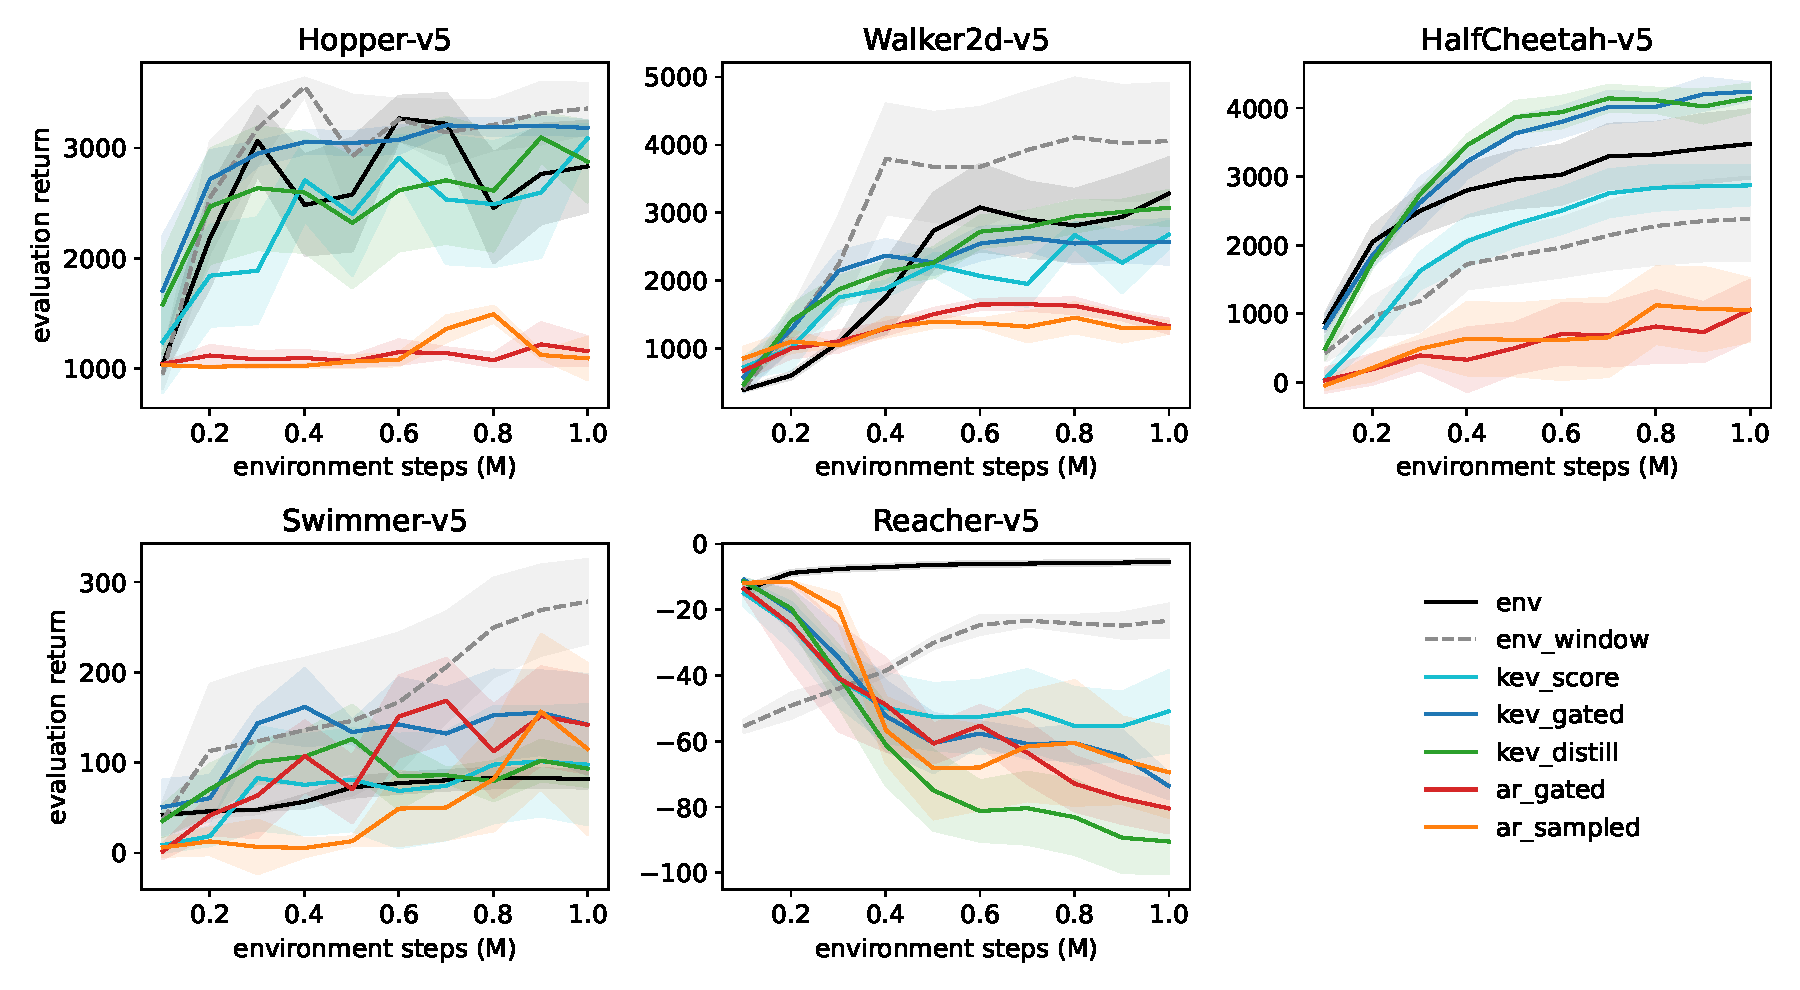
\includegraphics[width=\linewidth]{../../experiments/part1_control/results/learning_curves.pdf}
\caption{训练过程中的评估回报：每 $10^5$ 步评估 10 个回合，曲线为种子均值，阴影为 $\pm$ 一个标准误。}
\label{fig:curves}
\end{figure}

\paragraph{从汇总看，\kev{} 的门控奖励和蒸馏奖励接近工程化奖励，AR 评判的奖励则差得远。} 归一化分数的 IQM：\texttt{kev\_gated} 为 \NUM{iqm_kev_gated} \ci{\NUM{iqmlo_kev_gated}}{\NUM{iqmhi_kev_gated}}，\texttt{kev\_distill} 为 \NUM{iqm_kev_distill} \ci{\NUM{iqmlo_kev_distill}}{\NUM{iqmhi_kev_distill}}，\texttt{env} 为 \NUM{iqm_env} \ci{\NUM{iqmlo_env}}{\NUM{iqmhi_env}}，区间大幅重叠。在同一任务上，用这两种奖励训练的 run 胜过用工程化奖励训练的 run 的概率分别为 \NUM{pimpenv_kev_gated}（\texttt{kev\_gated}）和 \NUM{pimpenv_kev_distill}（\texttt{kev\_distill}）。去掉门控后，\kev{} 的分数表现更差（\NUM{iqm_kev_score} \ci{\NUM{iqmlo_kev_score}}{\NUM{iqmhi_kev_score}}，概率 \NUM{pimpenv_kev_score}）。AR 评判的奖励只达到工程化奖励归一化分数的三分之一左右：期望读出为 \NUM{iqm_ar_gated} \ci{\NUM{iqmlo_ar_gated}}{\NUM{iqmhi_ar_gated}}，采样读出为 \NUM{iqm_ar_sampled} \ci{\NUM{iqmlo_ar_sampled}}{\NUM{iqmhi_ar_sampled}}。在同一任务上，一个 \texttt{kev\_gated} run 胜过一个 \texttt{ar\_gated} run 的概率为 \NUM{pimp_all_kevgated_argated}；分任务看，Hopper 上为 \NUM{pimp_hopper_kevgated_argated}，HalfCheetah 上为 \NUM{pimp_cheetah_kevgated_argated}，Walker2d 上为 \NUM{pimp_walker_kevgated_argated}，而 Swimmer（\NUM{pimp_swimmer_kevgated_argated}）和 Reacher（\NUM{pimp_reacher_kevgated_argated}）上接近持平。

\paragraph{汇总掩盖了 Reacher。} IQM 去掉了最低和最高各四分之一的 run。均值更低：\texttt{kev\_gated} 为 \NUM{mean_kev_gated}，\texttt{kev\_distill} 为 \NUM{mean_kev_distill}。在 Reacher 上，每种评判奖励的最终结果都低于随机策略，因此这些 run 的归一化分数为负（表~\ref{tab:returns}）。所以我们逐个任务来看。

\paragraph{逐个任务。} 在 Hopper 上，\kev{} 的奖励最终接近工程化奖励（\texttt{kev\_gated} 为 \NUM{ret_hopper_kev_gated}，\texttt{env} 为 \NUM{ret_hopper_env}；改进概率 \NUM{pimp_hopper_kevgated_env}）。在 Walker2d 上它们更低（\texttt{kev\_gated} 为 \NUM{ret_walker_kev_gated}，\texttt{kev\_distill} 为 \NUM{ret_walker_kev_distill}，\texttt{env} 为 \NUM{ret_walker_env}；概率分别为 \NUM{pimp_walker_kevgated_env} 和 \NUM{pimp_walker_kevdistill_env}）。在 HalfCheetah 上，\texttt{kev\_gated}（\NUM{ret_cheetah_kev_gated}）和 \texttt{kev\_distill}（\NUM{ret_cheetah_kev_distill}）高于工程化奖励（\NUM{ret_cheetah_env}；两者的概率都是 \NUM{pimp_cheetah_kevgated_env}），原因见 \S\ref{sec:behaviour}。在 Swimmer 上，用工程化奖励训练的 PPO 几乎没让游动者动起来（\NUM{ret_swimmer_env}）；其他每种奖励的平均结果都更好，其中窗口平均的真实奖励最好（\NUM{ret_swimmer_env_window}），评判奖励在不同种子间差异很大。在 Reacher 上，只有工程化奖励学会了任务：用它为 \NUM{ret_reacher_env}，用它的窗口平均为 \NUM{ret_reacher_env_window}，用评判奖励为 \NUM{ret_reacher_kev_score} 到 \NUM{ret_reacher_kev_distill}。学习曲线显示，评判奖励训练的 Reacher 策略随着训练越来越差（图~\ref{fig:curves}）。

\paragraph{窗口级反馈在运动任务上代价很小，在 Reacher 上代价很大。} 在评判窗口上平均的真实奖励（\texttt{env\_window}）在汇总上至少不比逐步奖励差：IQM \NUM{iqm_env_window} \ci{\NUM{iqmlo_env_window}}{\NUM{iqmhi_env_window}}，改进概率 \NUM{pimpenv_env_window}。它在 Hopper（\NUM{pimp_hopper_envwindow_env}）、Walker2d（\NUM{pimp_walker_envwindow_env}）和 Swimmer（\NUM{pimp_swimmer_envwindow_env}）上领先；在 HalfCheetah 上落后（\NUM{pimp_cheetah_envwindow_env}），它的五个 run 中有 \NUM{flipruns_cheetah_env_window} 个最终翻成背朝下（\S\ref{sec:behaviour}）；在 Reacher 上也落后（\NUM{pimp_reacher_envwindow_env}）。一个 Reacher 回合只有两个 25 步的窗口，平均后的奖励不再告诉策略是哪些动作让指尖靠近了目标，其机械臂最终离目标并不比随机策略更近（表~\ref{tab:behaviour}）。因此，评判模型的时间分辨率能解释它们在 Reacher 上的部分失败，但完全解释不了 AR 评判在 Hopper 和 Walker2d 上的失败——在那里窗口平均奖励表现很好。

\paragraph{蒸馏只用十分之一的评判调用就保住了 \kev{} 的奖励。} \texttt{kev\_distill} 每个 run 只向评判模型询问 \NUM{judgewin_kev_distill} 个窗口，而不是 \NUM{judgewin_kev_gated} 个，最终与 \texttt{kev\_gated} 持平：IQM \NUM{iqm_kev_distill} 对 \NUM{iqm_kev_gated}，改进概率 \NUM{pimp_all_kevdistill_kevgated}。它最弱的任务是 Reacher（\NUM{ret_reacher_kev_distill}）。

\paragraph{训练中，两个评判模型的分数与奖励的相关程度相近。} 每个 run 对每次 rollout 记录了它所训练的窗口分数与同一批窗口的环境奖励之间的相关系数。对 rollout 和 run 取平均，\texttt{kev\_gated} 为 \NUM{traincorr_kev_gated}，\texttt{ar\_gated} 为 \NUM{traincorr_ar_gated}，而 \texttt{ar\_sampled} 只有 \NUM{traincorr_ar_sampled}——它的单次抽样大部分是噪声（\S\ref{sec:agreement}）。两种门控奖励与环境奖励的相关程度差不多，却训练出了截然不同的策略，下一节会说明这一点。

\subsection{策略学到了什么}\label{sec:behaviour}

回报并不说明策略做了什么。我们把每个最终策略在它的 20 个评估回合上重新运行一遍，记录机器人的实际行为（表~\ref{tab:behaviour}）。重新运行的回报与日志中的回报完全一致（最大差异 \NUM{beh_maxdiff}）。

\begin{table}[t]
\centering\small
\begin{tabular}{@{}lcccccc@{}}
\toprule
 & Hopper & Walker2d & Swimmer & HalfCheetah & \multicolumn{2}{c}{Reacher} \\ \cmidrule(lr){2-2}\cmidrule(lr){3-3}\cmidrule(lr){4-4}\cmidrule(lr){5-5}\cmidrule(l){6-7}
condition & still & still & still & runs flipped & effort & distance (m) \\ \midrule
\texttt{env} & 0\% & 1\% & 62\% & 1 of 5 & 0.01 & 0.101 \\
\texttt{env\_window} & 0\% & 0\% & 14\% & 3 of 5 & 0.19 & 0.180 \\
\texttt{kev\_score} & 0\% & 4\% & 11\% & 0 of 5 & 0.36 & 0.256 \\
\texttt{kev\_gated} & 1\% & 10\% & 15\% & 0 of 5 & 0.63 & 0.263 \\
\texttt{kev\_distill} & 1\% & 1\% & 11\% & 0 of 5 & 0.76 & 0.250 \\
\texttt{ar\_gated} & 49\% & 40\% & 18\% & 0 of 5 & 0.63 & 0.253 \\
\texttt{ar\_sampled} & 26\% & 17\% & 50\% & 0 of 3 & 0.56 & 0.252 \\ \midrule
random policy & 31\% & 4\% & 26\% & -- & 0.33 & 0.180 \\
\bottomrule
\end{tabular}

\caption{最终策略的行为，对回合和种子取平均（每个 run 20 个评估回合）。\emph{still}：$|v_x|<0.1$\,m/s 的步数占比。\emph{runs flipped}：猎豹有一半以上步数背朝下（$\cos(\text{pitch})<0$）的 run 数。\emph{effort}：动作平方的均值，取值于 $[0,1]$。\emph{distance}：一个回合中指尖到目标的平均距离。随机策略从均匀分布中采样动作。}
\label{tab:behaviour}
\end{table}

\begin{table}[t]
\centering\small
\begin{tabular}{@{}lcccccc@{}}
\toprule
 & & & \multicolumn{2}{c}{\kev{}} & \multicolumn{2}{c}{AR judge} \\ \cmidrule(lr){4-5}\cmidrule(l){6-7}
task & windows (slow / fast) & env.\ reward & progress & gated & progress & gated \\ \midrule
Hopper & 42 / 430 & 0.31 & 0.59 & 0.48 & 0.89 & 0.87 \\
Walker2d & 386 / 1238 & 0.27 & 0.62 & 0.47 & 0.90 & 0.87 \\
HalfCheetah & 309 / 1368 & $-$0.06 & 0.51 & 0.15 & 0.85 & 0.65 \\
\bottomrule
\end{tabular}

\caption{在 \S\ref{sec:agreement} 的窗口（\texttt{env} 条件的 run 记录的窗口）上，每种信号给“站着”相对于“跑”的报酬。表中数值为：未摔倒且慢于 \NUM{sf_slowmax}\,m/s 的窗口上的均值，除以快于 \NUM{sf_fastmin}\,m/s 的窗口上的均值。\emph{env.\ reward}：逐步环境奖励。}
\label{tab:slowfast}
\end{table}

\paragraph{AR 评判的奖励让单腿跳跃机器人和双足行走机器人学会了站着。} 最终的 \texttt{ar\_gated} 策略在 Hopper 上有 \NUM{still_hopper_ar_gated} 的步数站着不动，在 Walker2d 上为 \NUM{still_walker_ar_gated}。\texttt{kev\_gated} 的对应数字是 \NUM{still_hopper_kev_gated} 和 \NUM{still_walker_kev_gated}，\texttt{env} 为 \NUM{still_hopper_env} 和 \NUM{still_walker_env}。它们的平均前进速度为 \NUM{vx_hopper_ar_gated} 和 \NUM{vx_walker_ar_gated}\,m/s，而 \texttt{kev\_gated} 为 \NUM{vx_hopper_kev_gated} 和 \NUM{vx_walker_kev_gated}\,m/s，\texttt{env} 为 \NUM{vx_hopper_env} 和 \NUM{vx_walker_env}\,m/s。它们在 Hopper 上的回报（\NUM{ret_hopper_ar_gated}）接近 1000，也就是在一个 1000 步的回合里一直站着、仅靠存活奖励就能拿到的分数。对等级采样并不能消除这一现象：\texttt{ar\_sampled} 在两个任务上站着不动的步数占比为 \NUM{still_hopper_ar_sampled} 和 \NUM{still_walker_ar_sampled}。

表~\ref{tab:slowfast} 说明了原因。它比较每种信号给一个慢于 \NUM{sf_slowmax}\,m/s 的直立窗口和一个快于 \NUM{sf_fastmin}\,m/s 的窗口各付多少。AR 评判的门控分数在 Hopper 上给慢窗口的报酬是快窗口的 \NUM{sfratio_hopper_argated}（\NUM{sfs_hopper_argated} 对 \NUM{sff_hopper_argated}），在 Walker2d 上是 \NUM{sfratio_walker_argated}。工程化奖励只付 \NUM{sfratio_hopper_perstep} 和 \NUM{sfratio_walker_perstep}，\kev{} 的门控分数付 \NUM{sfratio_hopper_kevgated} 和 \NUM{sfratio_walker_kevgated}。回合中的每一步都得到其所在窗口的分数，而摔倒会结束回合。因此在 AR 评判的奖励下，直立站着每一步挣得几乎和跳跃一样多，又没有摔倒的风险。PPO 很早就找到了这一点：Hopper 上 \texttt{ar\_gated} 的曲线从第一次评估起就是平的（图~\ref{fig:curves}）。然而 AR 评判的分数对窗口的排序几乎和 \kev{} 一样好：它们与奖励的 Spearman 相关系数在 Hopper 上为 \NUM{rho_hopper_ar_gated} 对 \NUM{rho_hopper_kev_gated}，在 Walker2d 上为 \NUM{rho_walker_ar_gated} 对 \NUM{rho_walker_kev_gated}（表~\ref{tab:agreement}）。不同的是差距：AR 评判几乎把每个直立窗口都打在其分数范围的顶端。与奖励的排序一致性并没有预示出 PPO 能用上哪种奖励。

\paragraph{评判模型的奖励让猎豹保持直立。} 在 HalfCheetah 上，\texttt{env} 的五个 run 中有 \NUM{flipruns_cheetah_env} 个、\texttt{env\_window} 的五个 run 中有 \NUM{flipruns_cheetah_env_window} 个最终让猎豹背朝下。这是一个工程化奖励不加惩罚的局部最优。这些 run 的回报最多为 \NUM{flip_maxret}，而同样两种条件下保持直立的 run 至少为 \NUM{upright_minret}。用评判奖励训练的 \NUM{judge_runs_cheetah} 个 run 中没有一个翻倒。两个评判模型读到的任务描述都写明翻倒是不希望出现的，最低的 \texttt{progress} 等级也点了它的名。去掉翻倒的那个 run 后，\texttt{env} 在 HalfCheetah 上的平均回报为 \NUM{uprightret_env}，\texttt{kev\_gated} 为 \NUM{ret_cheetah_kev_gated}，所以 \kev{} 在这里的优势很大一部分来自翻倒。在这个例子里，评判模型的奖励带有工程化奖励所缺少的偏好，而策略遵循了它。

\paragraph{在 Reacher 上，评判模型的奖励让机械臂乱甩。} 用评判奖励训练的机械臂，指尖离目标的平均距离为 \NUM{dist_reacher_kev_distill} 到 \NUM{dist_reacher_kev_gated}\,m，比随机策略（\NUM{dist_reacher_random}\,m）和工程化奖励（\NUM{dist_reacher_env}\,m）都远。它们的控制力度也高于随机策略：\NUM{effort_reacher_kev_score} 到 \NUM{effort_reacher_kev_distill}，随机策略为 \NUM{effort_reacher_random}，\texttt{env} 为 \NUM{effort_reacher_env}。Reacher 的奖励每一步都按动作的平方扣分，这就是这些策略最终低于随机策略的原因。两个评判模型的分数跟随的是窗口内距离的变化（\kev{} 与 AR 评判的 \texttt{progress} 的 Spearman 相关系数分别为 \NUM{rhophys_reacher_kev_progress} 和 \NUM{rhophys_reacher_ar_progress}，\S\ref{sec:agreement}），而对 Reacher 奖励每一步都在计算的距离本身跟随得少得多（与奖励的相关系数为 \NUM{rho_reacher_kev_progress} 和 \NUM{rho_reacher_ar_progress}）。每个回合只有两个窗口，这两种信号都没能把 PPO 引到目标上。

\section{代价}\label{sec:cost}

\begin{table}[t]
\centering\small
\begin{tabular}{@{}lcccc@{}}
\toprule
condition & judged windows & judge wait (h) & wall-clock (h) & corr.\ (score, env reward) \\ \midrule
\texttt{env} & 0 & 0.0 & 0.1 & -- \\
\texttt{env\_window} & 0 & 0.0 & 0.1 & -- \\
\texttt{kev\_score} & 33{,}914 & 2.0 & 2.1 & 0.57 \\
\texttt{kev\_gated} & 33{,}942 & 1.9 & 2.1 & 0.56 \\
\texttt{kev\_distill} & 3{,}477 & 1.9 & 2.0 & 0.54 \\
\texttt{ar\_gated} & 33{,}861 & 1.9 & 2.0 & 0.52 \\
\texttt{ar\_sampled} & 33{,}869 & 1.9 & 2.0 & 0.17 \\
\bottomrule
\end{tabular}

\caption{每个 run 的代价，对任务和种子取平均：发送给评判模型的窗口数、等待其回答的时间、run 的总耗时，以及每次 rollout 中 run 所训练的窗口分数与同一批窗口的环境奖励之间相关系数的均值。一个 GPU 上的一个评判服务器同时服务最多 24 个 run，因此等待时间包含了它处理其他 run 请求的时间。}
\label{tab:cost}
\end{table}

表~\ref{tab:cost} 给出评判模型在每个 run 上的代价。对每个窗口都询问评判模型的 run，在 $10^6$ 步中大约发送 \NUM{judgewin_kev_gated} 个窗口，\texttt{kev\_distill} 大约发送 \NUM{judgewin_kev_distill} 个。不用评判模型的 run 耗时 \NUM{wallh_env}\,h；用评判模型的 run 耗时约 \NUM{wallh_kev_gated}\,h，约为前者的 \NUM{wallratio} 倍，其中几乎全部（\NUM{waith_kev_gated}\,h）花在等待评判上。这些时间反映的是我们的设置：一个 GPU 上的一个评判服务器同时回答最多 24 个 run 的请求，一个 run 的等待时间包含了服务器处理其他 run 请求的时间。这也是为什么 \texttt{kev\_distill} 只有十分之一的窗口，等待时间却差不多（\NUM{waith_kev_distill}\,h）：它的请求排在其他 run 的请求后面。我们没有测量评判模型只服务一个 run 的情形，而蒸馏奖励的节省会在那种情形下体现出来。

% 第一部分：讨论（由 main_zh.tex 引入）。

\section{讨论}\label{sec:discussion}

\paragraph{实验回答了什么。} 问题是：一个读取机器人行为文字摘要的 4B 评判模型，能否给 PPO 提供一个可以学习的奖励。用 \kev{} 的门控奖励或蒸馏奖励，PPO 在全部四个运动任务上都学会了向前运动：在 Hopper 上最终回报接近工程化奖励，在 HalfCheetah 上更高；在 Swimmer 上平均更高但分散很大，在 Walker2d 上更低。在 Reacher 上，每种评判奖励都失败了。同家族、同规模的自回归评判模型读的是同样的文本、回答的是同样的问题，但它的奖励让单腿跳跃机器人和双足行走机器人学会了站着。

\paragraph{相关性并不够。} 在 Hopper 和 Walker2d 上，两种门控评判按奖励给窗口排序的能力几乎一样好，无论是离线（\S\ref{sec:agreement}）还是训练中（表~\ref{tab:cost}）。然而一种奖励训练出了跳跃和行走，另一种训练出了站立。决定结果的是评判模型给任务想要的行为比给安全但无用的行为多付多少（表~\ref{tab:slowfast}）。把评判模型当作奖励进行离线检验时，除了相关系数，也应报告这个差距。在这里，摔倒会结束回合，而每一步都得到正的奖励，所以差距小时，存活比前进更划算；而分数挤在量表顶端的评判模型，正会让这个差距变小。

\paragraph{评判模型的奖励遵循的是任务描述。} 它不是工程化奖励的带噪副本。HalfCheetah 的任务描述说翻倒是不希望出现的，没有任何评判奖励让猎豹翻倒，而工程化奖励在五个 run 中有 \NUM{flipruns_cheetah_env} 个翻倒。Reacher 的任务描述要求控制力度尽量小，摘要里也报告了力度，可评判模型训练出的机械臂仍然乱甩。两个评判模型更多地跟随窗口内距离的变化，而不是距离的大小；每个回合只有两个窗口，PPO 没能找到目标。评判模型可以加入工程化奖励所缺少的偏好，也可能漏掉工程化奖励所收取的代价。

\paragraph{蒸馏。} 用 \kev{} 在十分之一窗口上的标签训练出的奖励网络，与对每个窗口都询问 \kev{} 的效果一样好。在我们的设置中，这一节省没有缩短 run 的时间，因为评判服务器是共享的。我们预计在评判模型只服务一个 run 时它会起作用，但没有测量。

\paragraph{局限。} 评判模型读的是我们根据仿真器特权状态设计的摘要，摘要点明了关键的物理量并给出了目标速度。这对评判模型有利，本实验对于从像素或原始观测进行评判没有任何结论。所有条件使用同一套 PPO 配置（CleanRL 的默认值）、$10^6$ 步、5 个种子（\texttt{ar\_sampled} 为 3 个）。置信区间很宽，各任务上介于约 0.3 和 0.7 之间的改进概率不应被解读为差异。AR 评判只用了一种提示格式和一种读出方式（在选项词元上取期望并重新归一化），没有校准，也不先推理再作答。换一种提示、校准或重新缩放读出、或先推理再作答，都可能改变它的差距；我们没有尝试，也没有为任何一个评判模型调提示。本文比较的是同一家族、同一规模的两个评判模型，并不能说明决策模型普遍比生成式评判模型更适合作为奖励。代价是在一个评判服务器被最多 24 个 run 共享的情况下测得的。最后，有 \NUM{resumed_runs} 个 run 在机器重置后恢复，每个丢失了一个回合。

\paragraph{与早期版本的关系。} 本文第 1--3 版报告了 \kev{} 奖励的排行榜和“对人类预言机 100\% 胜率”。这些结果并非由实验产生（见文首声明和 \file{CORRECTION.md}）。实测的答案要窄得多：加上门控或经过蒸馏后，\kev{} 的奖励在运动任务上接近工程化奖励；当任务描述带有工程化奖励所缺少的偏好时，它有帮助；在 Reacher 上它失败了；与同等规模的自回归评判模型的奖励相比，它对 PPO 有用得多。


\section*{可复现性}
所有 run 的代码、提示、配置、原始日志（每个训练回合、每次更新、每次评估，以及 2\% 被评判窗口的样本）和最终策略都在仓库中（\file{experiments/part1_control/}）。表格和正文中的每个数字都由 \file{dcjev/analysis/part1.py}、\file{dcjev/analysis/judge_agreement.py}、\file{dcjev/analysis/behaviour.py} 和 \file{dcjev/analysis/paper_numbers.py} 从中生成。

\bibliographystyle{plainnat}
\bibliography{../common/refs}
\end{document}
